\chapter{Using the Companion Labs}
\label{appB}

\begin{chapterintro}
The book comes with a body of runnable code: thirty-six interactive simulation labs, the
\emph{Lab Studio}, in which every idea of the book can be dragged, tuned and broken with a slider
while the plots update live; a compact signal-processing library called \texttt{commlib} that the
labs and the book's data figures share; and five GNU Radio flowgraphs that take the same experiments
onto an Ettus USRP B200. This appendix explains how to install it all on Windows, macOS or Linux,
gives a guided tour of a lab window, catalogues every lab and its experiments, walks through each
\texttt{commlib} module with short code examples, and shows how to test the code, write a lab of
your own and regenerate the book's figures. It ends with GNU Radio and the B200, used safely and
legally, and with fixes for the problems people actually run into.
\end{chapterintro}

%======================================================================
\section{What is in the box}
\label{sec:appB:overview}
%======================================================================

Reading about a matched filter is one thing; dragging a timing-offset slider and watching the eye
diagram close in front of you is another. The companion code exists for that second experience. It
lives in the folder \texttt{moderncomms-labs/}, next to the book's LaTeX sources, and has four parts
that are designed to be used together.

\begin{description}[leftmargin=1.2em,itemsep=3pt,font=\normalfont\bfseries]
\item[The labs] (\texttt{labs/labNN\_*.py}) are live desktop applications, one per topic, with
sliders and menus on the left, plots and big numerical readouts in the middle, and a short
explanation that follows your settings on the right. Each lab is a sequence of six to nine
\emph{experiments}, 286 in all, ordered as a story from the simplest picture to the ``wow''.
Nothing needs to be compiled and nothing runs in a browser: you start a lab with one
\texttt{python} command, or pick it from the gallery of Figure~\ref{fig:appB_launcher}.
\item[The Lab Studio] (\texttt{studio/}) is the small framework, built on Qt (PySide6) and
pyqtgraph, that turns a short, declarative Python file into such a window. You only need to know
about it if you want to write a lab of your own (Section~\ref{sec:appB:ownlab}).
\item[\texttt{commlib}] is the shared library: constellations and error-rate formulas, pulse shaping,
channel models, synchronisation loops, equalisers, OFDM, channel codes, MIMO, satellite geometry and
link budgets, spread spectrum and GNSS, line codes, RF impairments and more. It is deliberately
small and written to be read. When a lab calls \texttt{cl.gardner\_sync}, open
\texttt{commlib/sync.py} and look: the algorithm is a few dozen lines, written the way
Chapter~\ref{ch:sync} explains it.
\item[The GNU Radio flowgraphs] (\texttt{gnuradio/gr0N\_*.py}) are complete transmitters and receivers
for the USRP B200. Every one also runs \emph{without} hardware, through a software channel, so you
can study it before you own a radio.
\end{description}

\mdcfig[0.86]{appB_launcher}{The Lab Studio gallery (\texttt{python labs/launcher.py}). Every lab
is a card, grouped by the parts of the book, with its chapter numbers and a one-line summary of its
experiments; the search box filters as you type (``eye'', ``FM'', ``chapter 17''), and
\textsf{Launch} opens the lab in its own window. You can keep several open side by side.}

The same \texttt{commlib} also generates the data figures in this book (Section~\ref{sec:appB:figs}).
A BER curve in Chapter~\ref{ch:modulation} and the curve you watch build up in Lab~2 therefore come
from the same code, and if you find a discrepancy between the book and a lab, one of them has a bug
worth reporting.

\begin{keyidea}[Simulation first, hardware second]
Almost everything in this book can be learned, and most of it is best learned, in simulation. A
simulator lets you switch off one impairment at a time, run a billion bits overnight and compare
against theory exactly. Hardware then teaches the lessons a simulator cannot: that oscillators
drift, that the DC offset is real, that the spectrum is crowded. The labs are the core of the
course; the B200 experiments are the capstone.
\end{keyidea}

\begin{history}[From notebooks to a studio]
The first edition shipped its labs as Jupyter notebooks: pre-executed pages of code, text and
static figures, with a few sliders that came alive only inside a running kernel. Readers liked the
content and disliked the ceremony (start a server, open a browser, ``run all cells'', wait). The
second edition rebuilt every lab as a desktop application in which nothing is static: the moment
you move a control the plots, the numbers and even the explanatory text change. The physics and the
library underneath are the same; the notebooks are retired.
\end{history}

%======================================================================
\section{Repository layout}
\label{sec:appB:layout}
%======================================================================

\begin{figure}[htbp]\centering
\begin{tikzpicture}[font=\sffamily\small,
  box/.style={draw=navy,fill=navy!6,thick,rounded corners=2pt,minimum height=1.05cm,minimum width=3.3cm,align=center},
  core/.style={box,fill=accent!10,draw=accent,minimum width=3.4cm,minimum height=1.25cm},
  e/.style={-{Stealth[length=2.4mm]},thick,navy!70},
  l/.style={font=\sffamily\scriptsize,text=black!70,align=center}]
\node[core] (cl) at (0,0) {\texttt{commlib}\\{\scriptsize 47 modules of DSP}};
\node[box] (tests) at (0,2.5) {self-tests\\{\scriptsize\texttt{tests/}}};
\node[box] (labs) at (-5.0,1.25) {36 labs\\{\scriptsize\texttt{labs/labNN\_*.py}}};
\node[box] (studio) at (-5.0,-1.25) {Lab Studio\\{\scriptsize\texttt{studio/}: PySide6, pyqtgraph}};
\node[box] (figs) at (5.0,1.25) {book figures\\{\scriptsize\texttt{figscripts/chNN\_figs.py}}};
\node[box] (pdf) at (5.0,-1.25) {this book\\{\scriptsize\texttt{figs/*.pdf} $\to$ LaTeX}};
\node[box] (gr) at (0,-2.9) {GNU Radio flowgraphs\\{\scriptsize\texttt{gnuradio/gr0N\_*.py}}};
\node[box,minimum width=2.6cm] (b200) at (5.0,-2.9) {USRP B200\\{\scriptsize or \texttt{-{}-sim}}};
\draw[e] (labs.east) -- node[l,above=1pt]{all the DSP} (cl.west);
\draw[e] (labs) -- node[l,left]{window, controls,\\plots} (studio);
\draw[e] (figs.west) -- node[l,above=1pt]{same functions} (cl.east);
\draw[e] (figs) -- node[l,right]{vector PDFs} (pdf);
\draw[e] (gr) -- node[l,right]{Viterbi, file I/O} (cl);
\draw[e] (gr) -- (b200);
\draw[e] (tests) -- node[l,right]{41 tests} (cl);
\draw[e,dashed] (tests.west) -| node[l,above,pos=0.3]{every experiment, headless} (labs.north);
\draw[e,dashed] (studio.south) |- node[l,below,pos=0.75]{``Read more in the book'' opens the PDF} (-1.9,-1.95) -| (pdf.south);
\end{tikzpicture}
\caption{How the companion code fits together. Every arrow ends at \texttt{commlib}: the labs, the
book's figures and the GNU Radio flowgraphs all call the same functions, and the self-tests check
both the library and every lab experiment. The Lab Studio contains no signal processing at all;
it only draws what \texttt{commlib} computes.}
\label{fig:appB_pieces}
\end{figure}

\begin{lstlisting}[language={}]
comms-textbook/
  setup.sh                     one-time environment setup (Linux, macOS, WSL)
  book/                        LaTeX sources of this book
    figscripts/chNN_figs.py    one script per chapter; writes figs/chNN_*.pdf
    figscripts/figstyle.py     shared Matplotlib style; imports commlib
    build.sh, build_chapter.sh
  moderncomms-labs/
    README.md                  quick start and the list of labs
    LAB_STYLE_GUIDE.md         how to write or edit a lab
    requirements.txt           Python dependencies
    commlib/                   the shared DSP library (one module per topic)
    studio/                    the Lab Studio framework (PySide6 + pyqtgraph)
      README.md                its API, one page
    labs/
      launcher.py              START HERE: the gallery of all labs
      labNN_topic.py           one interactive lab per file (36 of them)
      _path.py                 makes commlib and studio importable
    gnuradio/
      grcommon.py              shared helpers: USRP or simulated channel
      gr01_ ... gr05_*.py      five hardware flowgraphs (all accept --sim)
    tests/
      test_commlib.py          library self-tests
      selftest_labs.py         every lab, headless, with screenshots
      screens/labNN/           the screenshots the self-test leaves behind
    data/                      IQ recordings (gr01 writes here) and data files
\end{lstlisting}

The \texttt{book/} and \texttt{moderncomms-labs/} folders must stay side by side: the figure scripts
find \texttt{commlib} through the relative path \texttt{../../moderncomms-labs}.
Figure~\ref{fig:appB_pieces} shows how the parts depend on one another. The arrows all point
towards \texttt{commlib}: it is the one place where signal processing lives, so the book, the labs
and the radio cannot drift apart.

%======================================================================
\section{Installation}
\label{sec:appB:install}
%======================================================================

\subsection{Requirements}

The labs need Python~3.10 or later and the packages in \texttt{requirements.txt}
(Table~\ref{tab:appB:reqs}). They are tested with both NumPy~1.x (from 1.24) and NumPy~2.x, on
Windows, macOS and Linux. Nothing else is required: no compiler, no GPU, no browser, no hardware. A
modest laptop runs every lab; the heavy parts (Monte Carlo error rates, decoder sweeps) run in a
background thread and draw their results as they arrive, so the window never freezes.

\begin{table}[htbp]\centering\small
\caption{Python packages used by the labs (\texttt{requirements.txt}).}\label{tab:appB:reqs}
\begin{tabular}{@{}lll@{}}
\toprule
Package & Minimum version & Used for\\
\midrule
numpy & 1.24 & all numerical work (1.x or 2.x)\\
scipy & 1.10 & filter design, special functions, sparse matrices, statistics\\
matplotlib & 3.7 & the book's figures (\texttt{commlib} imports it)\\
PySide6 & 6.5 & the Qt windows, controls and layout of the Lab Studio\\
pyqtgraph & 0.13.3 & the fast live plots inside the labs\\
\midrule
sounddevice & 0.4 & optional: audio for the \textsf{Listen} buttons\\
pypdf & 3.0 & optional: opens the book PDF at the exact page\\
\bottomrule
\end{tabular}
\end{table}

\subsection{The short version}

From the repository root, on any operating system:
\begin{lstlisting}[language=bash]
python -m venv .venv
# Windows PowerShell: .venv\Scripts\Activate.ps1
source .venv/bin/activate
pip install -r moderncomms-labs/requirements.txt
python moderncomms-labs/labs/launcher.py
\end{lstlisting}
The last line opens the gallery. If it does, you are done; the rest of this section covers the
details that differ between platforms.

\subsection{Windows}

Install Python~3.10 or later from \texttt{python.org} (tick ``Add python.exe to PATH'') or use
Anaconda/Miniconda. In PowerShell:
\begin{lstlisting}[language=bash]
cd comms-textbook
python -m venv .venv
.venv\Scripts\Activate.ps1          # cmd.exe: .venv\Scripts\activate.bat
pip install -r moderncomms-labs\requirements.txt
python moderncomms-labs\labs\launcher.py
\end{lstlisting}
If PowerShell refuses to run the activation script, allow local scripts once with
\begin{lstlisting}[language=bash]
Set-ExecutionPolicy -Scope CurrentUser RemoteSigned
\end{lstlisting}
\begin{sloppypar}
Git Bash works too, with the Linux commands; there the activation line is
\texttt{source .venv/Scripts/activate}. Audio works out of the box through Windows' built-in
\texttt{winsound}. On a high-resolution laptop screen the windows scale with your Windows display
setting; see Section~\ref{sec:appB:trouble} if they come out too large or too small.
\end{sloppypar}

\subsection{macOS and Linux}

\begin{lstlisting}[language=bash]
cd comms-textbook
python3 -m venv .venv
source .venv/bin/activate
pip install --upgrade pip
pip install -r moderncomms-labs/requirements.txt
python moderncomms-labs/labs/launcher.py
\end{lstlisting}
On macOS, use a Python from \texttt{python.org}, Homebrew (\texttt{brew install python}) or conda
rather than the system Python; sound plays through the built-in \texttt{afplay}. On Debian and
Ubuntu, \texttt{sudo apt install python3-venv} provides the \texttt{venv} module if it is missing,
and Qt~6 needs one system library that minimal installations lack,
\texttt{sudo apt install libxcb-cursor0}. Sound uses \texttt{paplay} or \texttt{aplay} if present.
Windows Subsystem for Linux works through WSLg on Windows~11, but a native Windows install is
smoother for the labs. From the repository root, \texttt{./setup.sh} creates one virtual environment
for the whole project, checks the LaTeX tool chain needed to build the book and runs the self-tests.

\mdcpairany{appB_lab14_bessel}{Lab~14, experiment~4: the spectrum of tone-modulated FM. Drag the
modulation index and watch the carrier line (red) vanish at $\beta=2.405$, the first Bessel null of
Appendix~\ref{appA}; the shaded band is Carson's rule. Lab~14's stereo experiment also lets you
\emph{listen}.}{appB_lab16_mulaw}{Lab~16, experiment~5: G.711 $\mu$-law. Top left: SQNR versus talker
level for uniform and companded quantisers; top right: the 8-chord compressor; bottom: the coding
error of a real waveform. \textsf{Listen through the codec} plays it.}

\subsection{Conda}

With Anaconda, Miniconda or Miniforge, a dedicated environment keeps the labs separate from
everything else:
\begin{lstlisting}[language=bash]
conda create -n mdc -c conda-forge python=3.12 numpy scipy matplotlib \
             pyside6 pyqtgraph
conda activate mdc
\end{lstlisting}
If you will use GNU Radio, install \emph{radioconda} instead (Section~\ref{sec:appB:gnuradio}) and add
the lab packages to it with \texttt{conda}/\texttt{mamba}, not \texttt{pip}, so that conda remains in
charge of NumPy.

\subsection{Checking that it works}

Two commands confirm the installation without opening a single window:
\begin{lstlisting}[language=bash]
cd moderncomms-labs
python tests/test_commlib.py          # library: every test prints PASS
python tests/selftest_labs.py lab03   # one lab, headless: RESULT lab03: PASS
\end{lstlisting}
Section~\ref{sec:appB:rebuild} explains what they check.

%======================================================================
\section{Running a lab: a guided tour}
\label{sec:appB:running}
%======================================================================

\subsection{Starting a lab}

The easiest door is the gallery: \texttt{python labs/launcher.py} (from \texttt{moderncomms-labs/};
\texttt{python -m studio} does the same). To open one lab directly, run its file:
\begin{lstlisting}[language=bash]
cd moderncomms-labs
python labs/lab03_pulse_shaping.py              # open the lab
python labs/lab03_pulse_shaping.py --exp 3      # open on experiment 3
python labs/lab03_pulse_shaping.py --dark       # dark theme (remembered)
\end{lstlisting}
A lab can be started from any folder (\texttt{labs/\_path.py} finds \texttt{commlib} and
\texttt{studio} for it), and it remembers the last experiment you looked at, your theme and the
challenges you have completed. Table~\ref{tab:appB:cli} lists every command-line option; the last
three are for testing and for making screenshots like the ones in this appendix.

\begin{table}[htbp]\centering\small
\caption{Command-line options shared by every lab.}\label{tab:appB:cli}
\begin{tabularx}{\linewidth}{@{}>{\ttfamily}l>{\raggedright\arraybackslash}X@{}}
\toprule
\normalfont Option & Effect\\
\midrule
-{}-exp N & open on experiment N (1-based)\\
-{}-dark & start in the dark theme (the choice is remembered)\\
-{}-shot FILE & open experiment \texttt{-{}-exp}, save a screenshot of the window to FILE and quit\\
-{}-smoke S & visit every experiment, quit after S seconds and print \texttt{SMOKE OK}\\
-{}-selftest & headless test of every experiment at default and random settings, with screenshots
(add \texttt{-{}-random K}, \texttt{-{}-out DIR}, \texttt{-{}-dark})\\
\bottomrule
\end{tabularx}
\end{table}

\subsection{A tour of the window}

Every lab looks and works the same way, so once you know one you know them all.
Figure~\ref{fig:appB_tour} shows Lab~3 open on its live eye diagram, with the parts numbered.

\mdcfig[1.0]{appB_tour}{The anatomy of a lab window (Lab~3, experiment~3, \emph{Live eye diagram}).
The numbers match the list in the text: (1)~experiments, (2)~controls, (3)~readouts, (4)~live plots,
(5)~\emph{What's going on}, (6)~\emph{Try this} challenges, (7)~the book link, (8)~Play/Pause,
(9)~Reset, Export PNG, theme and notes, (10)~the status bar.}

\begin{enumerate}[leftmargin=1.6em,itemsep=3pt,label=\textbf{\arabic*}]
\item \textbf{Experiments.} The lab's six to nine experiments, in story order. Click one, or use
Ctrl+1\ldots9 and PgUp/PgDn. Each experiment is a self-contained page with its own controls and
plots.
\item \textbf{Controls.} Sliders, button groups, menus, switches and text boxes, grouped under
headings such as \textsc{Transmitter}, \textsc{Channel} and \textsc{Receiver}. Every slider shows
its value and unit; type into the value to set it exactly, or double-click the slider to reset it.
Hover over a control for a one-line explanation of what it physically is. Controls that make no
sense in the current mode grey out.
\item \textbf{Readouts.} The three or four numbers an engineer would put on a slide: eye height, SNR,
bit error rate, bandwidth. A readout turns green or red when there is a clear target, and shows
``$<10^{-12}$'' or ``---'' rather than a meaningless number.
\item \textbf{Live plots.} They redraw within a few tens of milliseconds of any change, so you can
\emph{scrub} a slider and watch cause and effect. Drag to pan, scroll to zoom, right-click for the
plot menu; some plots also respond to clicks (flip a bit in the Viterbi trellis of Lab~8) or have
handles you can drag (the floors of the water-filling vessel in Lab~19).
\item \textbf{What's going on.} Two to four short paragraphs that explain what you are looking at
\emph{for your current settings}: ``Right now the eye is \emph{wide open}: 89\,\% of its ideal height
\ldots''. Move a control and the text changes with the plots. A shaded box at the end holds the one
idea to keep. F1 hides the panel when you want more room for plots.
\item \textbf{Try this.} Two to four challenges per experiment, each with a number in it (``Keep
the eye at least 50\,\% open with $E_s/N_0$ of 19\,dB or less''). They tick themselves when you
achieve them, and the lab remembers which ones you have done. None is true at the default
settings, and most require finding a trade-off rather than pushing a slider to its end. Hover over
a challenge for a hint.
\item \textbf{Read more in the book.} The section of this book that explains the experiment, with its
number and page. Click it and the PDF opens at that section (with \texttt{pypdf} installed the page
is exact in every browser and in SumatraPDF or Adobe Reader; other viewers open at the start and the
status bar names the page).
\item \textbf{Play/Pause.} Streaming experiments (an oscilloscope-style eye, a satellite pass, a
fading envelope, a live Erlang switchboard; 52 experiments in all) run continuously with fresh
noise every frame. Pause (Ctrl+P) freezes the picture so you can study it.
\item \textbf{Toolbar.} \textsf{Reset} (Ctrl+R) restores the experiment's defaults. \textsf{Export PNG}
(Ctrl+E) saves the plot area as an image, named after the lab and experiment, for a report or a
slide. \textsf{Dark}/\textsf{Light} (Ctrl+D) switches theme. \textsf{Hide notes} (F1) folds away the
right-hand panel.
\item \textbf{Status bar.} Messages (``Background computation finished in 0.6\,s'') and the time the
last update took.
\end{enumerate}

\begin{inpractice}[How to get the most from a lab]
Predict before you move. Before you drag a slider, say out loud what you expect to see: the shape
of the spectrum, the BER at 6\,dB, whether the loop will lock. The surprises are where the learning
is. Then change one thing at a time, and use \textsf{Reset} freely. Read the \emph{What's going on}
panel \emph{after} you have looked at the plots, not before. Finally, when a lab calls a library
function you have not met, open its source in \texttt{commlib}: the labs are designed so that you
could rewrite the library from them.
\end{inpractice}

\subsection{Experiments that run, sound and remember}

Some experiments do more than redraw. Those that need many random trials, such as a Monte Carlo
bit-error-rate curve, run them in a \emph{background} thread and draw each point as it arrives
(Lab~2, experiment~5 in Figure~\ref{fig:appB_lab02_ber}); move a control and the run restarts at once.
Labs~14, 15, 16, 18, 24 and 34 have \textsf{Listen} buttons: hear FM stereo, an AM station through
a superheterodyne, speech through a $\mu$-law codec, the Doppler whistle of a passing satellite, an
LPC vocoder, or your own message in Morse. Sound uses \texttt{sounddevice} if it is installed and
otherwise the operating system's player; nothing is downloaded, every sound is synthesised by the
lab. Some experiments accept your own input: type a message to be keyed in Morse (Lab~34) or
compressed (Labs~19 and~24), or a bit pattern to be line-coded (Lab~13).

\mdcpairany{appB_lab03_dark}{The dark theme (Ctrl+D or \texttt{-{}-dark}), here on Lab~3's
\emph{NRZ versus PAM-4}: two bits per symbol at half the rate, three eyes each a third of the height,
over the same lossy backplane.}{appB_lab19_waterfill}{Lab~19, experiment~8: water-filling with your
hands. Drag a sub-channel's floor and the water (power) redistributes; the bars below compare
equal power, water-filling and integer bit loading. Compare Figure~\ref{fig:appA_waterfill}.}

\begin{table}[htbp]\centering\small
\caption{Keyboard shortcuts in every lab window.}\label{tab:appB:keys}
\begin{tabular}{@{}ll@{\qquad}ll@{}}
\toprule
Keys & Action & Keys & Action\\
\midrule
Ctrl+1 \ldots\ Ctrl+9 & go to experiment 1--9 & Ctrl+R & reset the experiment\\
PgUp / PgDn & previous / next experiment & Ctrl+E & export the plots as PNG\\
Ctrl+P & play / pause & Ctrl+D & dark / light theme\\
F1 & hide / show the notes panel & double-click slider & reset that control\\
\bottomrule
\end{tabular}
\end{table}

%======================================================================
\section{Self-tests: keeping the labs honest}
\label{sec:appB:rebuild}
%======================================================================

Two test programs guard the code. The first checks the library:
\begin{lstlisting}[language=bash]
python tests/test_commlib.py        # or: python -m pytest -q tests/test_commlib.py
\end{lstlisting}
Its 41 tests check that simulated QPSK, 16-QAM and 64-QAM error rates match theory, that LLR signs
are consistent, that RRC filters satisfy the Nyquist criterion, that the Gardner and
Mueller--M\"uller timing loops and the carrier PLL converge, that the equalisers, the OFDM chain and
LS channel estimation work, that Viterbi decoding (single and batched) and LDPC and polar decoding
correct errors, that the PEG LDPC construction has no 4-cycles, and that each topic module
(information theory, block codes, CPM, propagation, source coding, the LTE/NR PHY, RF models,
analog modulation, fading, PCM, the superheterodyne, multirate DSP, spread spectrum and the rest)
reproduces numbers quoted in the book. Run it after any change to \texttt{commlib}.

The second exercises every lab, headless:
\begin{lstlisting}[language=bash]
python tests/selftest_labs.py                 # every lab, one process each
python tests/selftest_labs.py lab03 lab14     # some labs
python tests/selftest_labs.py --random 2      # fewer random settings (faster)
python labs/lab03_pulse_shaping.py --selftest # one lab; add --dark for the dark theme
\end{lstlisting}
For each experiment it builds the page, runs it at the default settings (including background jobs
in a quick mode and a few animation frames), then at several random settings of every control, and
re-checks the challenges each time. It fails on any exception, on infinite numbers in a readout or a
plot, and on an update slower than half a second. It runs with Qt's \texttt{offscreen} platform, so
it works over SSH and in continuous integration, and it saves a screenshot of every experiment to
\texttt{tests/screens/labNN/} (Figure~\ref{fig:appB_selftest}). Look at them: a clipped label or a
legend over the data is a bug too.

\mdcfig[1.0]{appB_selftest}{What the self-test leaves behind: one screenshot per experiment, here the
eight of Lab~3 at their default settings (\texttt{tests/screens/lab03/}). A second set,
\texttt{*\_random.png}, shows each experiment at the last random setting tried, which is where
layout bugs tend to hide.}

%======================================================================
\section{The lab catalogue}
\label{sec:appB:catalogue}
%======================================================================

Tables~\ref{tab:appB:labs1}--\ref{tab:appB:labs5} list all 36 labs in the order of the book's
chapters, the same order as the gallery, with the title of every experiment. The lab numbers
follow the order in which the labs were first written, not the chapter order, so use the chapter
column (or the paths below) to choose what to run next. Each chapter's \emph{Simulation lab} box
names the matching file, and many \emph{Try it} boxes in the text point to a specific experiment
and slider.

\begin{table}[htbp]\centering\footnotesize
\caption{The companion labs, part 1: foundations and signal processing for radio (Chapters 1--7). The number in brackets is the number of experiments.}\label{tab:appB:labs1}
\renewcommand{\arraystretch}{1.12}
\begin{tabularx}{\linewidth}{@{}rl>{\raggedright}p{0.30\linewidth}>{\raggedright\arraybackslash}X@{}}
\toprule
Lab & Ch. & Title and file & Experiments\\
\midrule
34 & 1 & \textbf{The Telegraph and the Birth of Signalling}\newline\texttt{lab34\_\allowbreak{}telegraph\_\allowbreak{}history.py} & Morse keying and key clicks; Morse versus Huffman; Kelvin's Atlantic cable; Chappe's semaphore pipeline; Repeaters vs regenerators; Loading the telephone line; Capacity: semaphore to modem (7)\\
35 & 2 & \textbf{Fourier, Spectra and Bandwidth}\newline\texttt{lab35\_\allowbreak{}fourier\_\allowbreak{}spectra.py} & Fourier series builder; Windows, leakage and scalloping; Zero padding is not resolution; The uncertainty principle; Convolution in slow motion; Phase delay, group delay, dispersion; Five bandwidths of one signal; The spectrogram (STFT); Two-tone test and IP3 (9)\\
1 & 2, 7 & \textbf{Complex Baseband and IQ Sampling}\newline\texttt{lab01\_\allowbreak{}baseband.py} & The IQ helix; Why two ADCs: real vs IQ sampling; Up- and down-conversion; The digital down-converter; Zero-IF fingerprints: DC and I/Q images; Oscillator phase noise; ADC bits, back-off and processing gain; Sensitivity and range; A live waterfall (9)\\
33 & 3 & \textbf{Noise and Detection}\newline\texttt{lab33\_\allowbreak{}noise\_\allowbreak{}detection.py} & Why noise is Gaussian; The Q-function and the tails; Rayleigh and Rice envelopes; Filtered noise and its bandwidth; Bandpass noise: two baseband halves; Friis: who adds the noise?; The Y-factor measurement; Detection: thresholds and ROC curves; Finding a signal below the noise (9)\\
14 & 4 & \textbf{Analog Modulation: AM, SSB, FM and Stereo}\newline\texttt{lab14\_\allowbreak{}analog\_\allowbreak{}am\_\allowbreak{}fm.py} & AM and the envelope detector; DSB-SC and SSB; FM: frequency follows the message; FM spectrum: Bessel and Carson; FM noise, clicks and the threshold; FM stereo multiplex (6)\\
15 & 4, 7 & \textbf{The Superheterodyne Receiver}\newline\texttt{lab15\_\allowbreak{}superhet\_\allowbreak{}receiver.py} & Tune the superhet; The image problem; IF selectivity; AGC: the receiver's iris; Double conversion; Intermod, blocking and SFDR; Zero-IF vs low-IF (7)\\
16 & 5 & \textbf{Sampling, PCM and Companding}\newline\texttt{lab16\_\allowbreak{}pcm\_\allowbreak{}companding.py} & Sampling and aliasing; Reconstruction and ZOH droop; Quantization: bits and SQNR; Dither; $\mu$-law and A-law (G.711); Delta modulation and CVSD; Sigma-delta noise shaping; Clock jitter limits SNR; T1 and E1 frames (9)\\
17 & 6 & \textbf{Digital Filters and Multirate DSP}\newline\texttt{lab17\_\allowbreak{}multirate\_\allowbreak{}dsp.py} & Pole--zero playground; FIR design: windows vs equiripple; IIR filters: sharp, cheap, fragile; Decimation, interpolation, aliasing; Polyphase channelizer; CIC decimator and compensator; NCO: phase bits, spurs, dither; CORDIC: rotation by shifts; A complete digital down-converter (9)\\
36 & 7 & \textbf{The RF Transceiver}\newline\texttt{lab36\_\allowbreak{}rf\_\allowbreak{}transceiver.py} & Two-tone test and IIP3; Receiver line-up builder; Phase noise and reciprocal mixing; I/Q imbalance and the image; Power amplifier: ACLR and EVM; PA classes, Doherty and ET; Crest-factor reduction; Digital predistortion (8)\\
\bottomrule
\end{tabularx}
\end{table}

\subsection{A tour in pictures}

The screenshots on the next pages, all taken from the labs at or near their default settings, give
a feel for the range: block diagrams you can click, streaming oscilloscopes, maps, spectrograms and
Monte Carlo curves that grow while you watch.

\mdcpairany{appB_lab34_cable}{Lab~34, \emph{Kelvin's Atlantic cable}: a telegraph pulse smeared by
3000\,km of RC line. Load the 1858 or 1866 cable and find the fastest keying speed that stays
readable; the law of squares (bottom right) explains why.}{appB_lab35_fourier}{Lab~35, \emph{Fourier
series builder}: add harmonics one at a time and watch a square wave assemble, ringing at the jumps
(the Gibbs overshoot never falls below 9\,\% of the jump).}

\mdcpairany{appB_lab17_pz}{Lab~17, \emph{Pole--zero playground}: drag poles and zeros around the
unit circle and see the magnitude and impulse responses follow, the geometry of
Figure~\ref{fig:appA_zplane} made live.}{appB_lab33_tails}{Lab~33, \emph{The Q-function and the
tails}: a Gaussian tail beyond a threshold, its bounds, and a Monte Carlo estimate that runs out of
samples just where the interesting error rates begin.}

\begin{table}[htbp]\centering\footnotesize
\caption{The companion labs, part 2: digital transmission (Chapters 8--12).}\label{tab:appB:labs2}
\renewcommand{\arraystretch}{1.12}
\begin{tabularx}{\linewidth}{@{}rl>{\raggedright}p{0.30\linewidth}>{\raggedright\arraybackslash}X@{}}
\toprule
Lab & Ch. & Title and file & Experiments\\
\midrule
3 & 8 & \textbf{Pulse Shaping, Nyquist and the Eye}\newline\texttt{lab03\_\allowbreak{}pulse\_\allowbreak{}shaping.py} & Pulses and their spectra; Nyquist: zero ISI; Live eye diagram; The matched filter; Matched and mismatched chains; BER: simulation meets theory; NRZ versus PAM-4; Faster than Nyquist (8)\\
13 & 8 & \textbf{Line Codes, Jitter and SerDes Eyes}\newline\texttt{lab13\_\allowbreak{}line\_\allowbreak{}codes\_\allowbreak{}eyes.py} & Line codes \& spectra; Spectral lines \& DC wander; Scramblers; 8b/10b running disparity; Eyes \& bathtub; PAM-4 over a lossy channel; Duobinary \& precoding (7)\\
2 & 9 & \textbf{Digital Modulation and Optimal Detection}\newline\texttt{lab02\_\allowbreak{}modulation.py} & Constellation gallery; From waveforms to points; Noise and decision regions; Priors move the boundary; BER: Monte Carlo vs theory; Soft bits: LLRs; Orthogonal FSK, noncoherently; The bandwidth--power plane; Rayleigh fading and diversity (9)\\
21 & 9 & \textbf{Constant Envelope, PAPR and EVM}\newline\texttt{lab21\_\allowbreak{}cpm\_\allowbreak{}evm.py} & Phase that remembers; Spectra and 99 \% bandwidth; MSK is offset QPSK; Three receivers; Envelope and PAPR; Through a saturating amplifier; EVM: impairment signatures; An EVM budget for 1024-QAM (8)\\
4 & 10 & \textbf{Synchronization: Carrier, Timing and Frame}\newline\texttt{lab04\_\allowbreak{}synchronization.py} & What each error looks like; Inside the PLL; Phase detector S-curves; A Costas loop locks on; Frequency estimators vs the bound; Symbol timing recovery; Interpolators and Farrow; Finding the frame; OFDM timing and cell search (9)\\
5 & 11 & \textbf{The Wireless Channel}\newline\texttt{lab05\_\allowbreak{}channels.py} & Path loss and shadowing; Standing waves in a room; Doppler: driving through the speckle; Rayleigh, Rice and Nakagami; Echoes become notches; 3GPP channel models in motion; Error rate in fading, and diversity; Sounding a channel (8)\\
22 & 11 & \textbf{Propagation and Link Budgets}\newline\texttt{lab22\_\allowbreak{}propagation\_\allowbreak{}link\_\allowbreak{}budget.py} & Friis: free space and antennas; The decibel bank account; Fresnel zones and knife edges; Two rays and the breakpoint; Hata, COST-231 and 3GPP 38.901; Rain and oxygen; Edge coverage vs area coverage; A coverage map (8)\\
6 & 12 & \textbf{Equalization}\newline\texttt{lab06\_\allowbreak{}equalization.py} & Symbols that collide; Zero forcing vs MMSE; Equalizer length and delay; LMS learning, live; LMS vs RLS: eigenvalue spread; Blind equalization: CMA; Decision feedback and error bursts; MLSE: the Viterbi equalizer; SerDes: CTLE, FFE and DFE (9)\\
\bottomrule
\end{tabularx}
\end{table}

\mdcpairany{appB_lab02_gallery}{Lab~2, \emph{Constellation gallery}: 16-QAM with its Gray labels, and
(right) the whole zoo of constellations ranked by distance per bit against peak power.}{appB_lab02_ber}{Lab~2,
\emph{BER: Monte Carlo vs theory}: red circles are simulated points, computed in the background
and drawn as they arrive, landing on the theoretical curve.}

\begin{table}[htbp]\centering\footnotesize
\caption{The companion labs, part 3: information and coding (Chapters 13--16).}\label{tab:appB:labs3}
\renewcommand{\arraystretch}{1.12}
\begin{tabularx}{\linewidth}{@{}rl>{\raggedright}p{0.30\linewidth}>{\raggedright\arraybackslash}X@{}}
\toprule
Lab & Ch. & Title and file & Experiments\\
\midrule
19 & 13 & \textbf{Information Theory}\newline\texttt{lab19\_\allowbreak{}information\_\allowbreak{}theory.py} & Surprise and entropy; Entropy of text and images; Huffman coding; DMC capacity; Shannon's AWGN limit; Constrained capacity; Finite blocklength; Water-filling; Rate--distortion (9)\\
8 & 14 & \textbf{Convolutional Codes and the Viterbi Algorithm}\newline\texttt{lab08\_\allowbreak{}convolutional.py} & How far is perfect?; The shift-register encoder; Trellis and free distance; Viterbi, step by step; Hard against soft decisions; Puncturing: one decoder, many rates; Traceback depth and quantisation; Bursts, CRC and interleaving (8)\\
20 & 14 & \textbf{Block Codes: Hamming to Reed--Solomon}\newline\texttt{lab20\_\allowbreak{}block\_\allowbreak{}codes.py} & Hamming (7,4) on a Venn diagram; SECDED: guarding memory; A CRC calculator; What a CRC can and cannot see; The GF(2$^m$) playground; Reed--Solomon: errors, erasures, the cliff; Interleaving against bursts; Coding gain at your target (8)\\
9 & 15 & \textbf{LDPC and Polar Codes}\newline\texttt{lab09\_\allowbreak{}ldpc\_\allowbreak{}polar.py} & Tanner graph and short cycles; Belief propagation, live; Sum-product against min-sum; Iterations and early stopping; Channel polarization; SC against CRC-aided list decoding; Short blocks and the finite-length limit (7)\\
23 & 15 & \textbf{Turbo Codes and EXIT Charts}\newline\texttt{lab23\_\allowbreak{}turbo\_\allowbreak{}exit.py} & Recursive encoders and the interleaver; BCJR: log-MAP against max-log; Turbo decoding, iteration by iteration; EXIT chart: watch the tunnel open; Density evolution on the erasure channel; Spatial coupling: the decoding wave; The error floor and the interleaver (7)\\
24 & 16 & \textbf{Source Coding}\newline\texttt{lab24\_\allowbreak{}source\_\allowbreak{}coding.py} & Huffman vs arithmetic coding; LZ77: the sliding window; Quantisers and Lloyd--Max; DCT energy compaction; A toy JPEG; LPC: a buzz and a filter; Masking: hide a tone; Noise under the mask; Motion estimation (9)\\
\bottomrule
\end{tabularx}
\end{table}

\begin{table}[htbp]\centering\footnotesize
\caption{The companion labs, part 4: systems (Chapters 17--20).}\label{tab:appB:labs4}
\renewcommand{\arraystretch}{1.12}
\begin{tabularx}{\linewidth}{@{}rl>{\raggedright}p{0.30\linewidth}>{\raggedright\arraybackslash}X@{}}
\toprule
Lab & Ch. & Title and file & Experiments\\
\midrule
7 & 17 & \textbf{OFDM: From the IFFT to the NR Grid}\newline\texttt{lab07\_\allowbreak{}ofdm.py} & Orthogonal subcarriers; Building a symbol: IFFT + CP; Cyclic prefix vs multipath; The one-tap equaliser; Acquisition: Schmidl \& Cox; Pilots and channel estimation; PAPR: OFDM vs DFT-s-OFDM; 5G NR numerology explorer (8)\\
28 & 17 & \textbf{OFDM as a System}\newline\texttt{lab28\_\allowbreak{}ofdm\_\allowbreak{}system.py} & Channel estimation: LS, DFT, LMMSE; Frequency offset, Doppler, phase noise; Coded OFDM and interleaving; Clipping, filtering and the PA; WOLA and filtered OFDM; DMT on copper: bit loading; OFDM as a radar (7)\\
25 & 18 & \textbf{Spread Spectrum, CDMA and GPS}\newline\texttt{lab25\_\allowbreak{}spread\_\allowbreak{}spectrum\_\allowbreak{}gps.py} & PN, Gold and Kasami codes; DSSS against a jammer; Frequency hopping; The RAKE receiver; CDMA: near--far and multiuser detection; GPS acquisition; DLL and PLL tracking; Position fix and DOP (8)\\
10 & 19 & \textbf{MIMO: Diversity, Capacity, Detection}\newline\texttt{lab10\_\allowbreak{}mimo.py} & Fading branches, live; SC, EGC and MRC error rates; Alamouti versus MRC; Eigen-channels and water-filling; Ergodic and outage capacity; ZF, MMSE, SIC and ML; The diversity--multiplexing trade-off; Massive MIMO: channel hardening; MU-MIMO precoding: MR, ZF, RZF (9)\\
29 & 19 & \textbf{Antenna Arrays and Beamforming}\newline\texttt{lab29\_\allowbreak{}arrays\_\allowbreak{}beamforming.py} & Steer a line of antennas; A planar panel and its EIRP; Beam squint: phase vs true delay; Direction finding: MUSIC \& co; SSB beam sweep and codebook; Hybrid precoding by OMP; Line-of-sight MIMO spacing (7)\\
26 & 20 & \textbf{The Cellular Concept}\newline\texttt{lab26\_\allowbreak{}cellular\_\allowbreak{}system.py} & Clusters, reuse and SIR; Erlang: a live switchboard; ALOHA and CSMA, live; Slotted ALOHA's instability; Wi-Fi's DCF: Bianchi's model; RACH collisions and barring; Stochastic geometry: PPP coverage; Proportional fair scheduling; Handover: hysteresis and TTT (9)\\
11 & 20, 21, 22 & \textbf{Air Interfaces: Cells, Trunks, Schedulers}\newline\texttt{lab11\_\allowbreak{}air\_\allowbreak{}interfaces.py} & Frequency reuse and SIR; Trunking: a live switchboard; OFDMA scheduling, live; Link adaptation and HARQ; Wi-Fi contention, live; 4096-QAM: the EVM budget; Air interfaces side by side (7)\\
\bottomrule
\end{tabularx}
\end{table}

\begin{table}[htbp]\centering\footnotesize
\caption{The companion labs, part 5: systems (Chapters 21--25).}\label{tab:appB:labs5}
\renewcommand{\arraystretch}{1.12}
\begin{tabularx}{\linewidth}{@{}rl>{\raggedright}p{0.30\linewidth}>{\raggedright\arraybackslash}X@{}}
\toprule
Lab & Ch. & Title and file & Experiments\\
\midrule
27 & 21 & \textbf{Inside an LTE/NR Downlink}\newline\texttt{lab27\_\allowbreak{}lte\_\allowbreak{}nr\_\allowbreak{}phy.py} & The resource grid builder; PSS and SSS: why they work; Cell search on two cells; The PDSCH chain, step by step; HARQ: chase vs incremental redundancy; CQI, MCS and throughput; Peak-rate calculator (TS 38.306) (7)\\
31 & 22 & \textbf{Wi-Fi, Bluetooth LE, 802.15.4, LoRa and RFID}\newline\texttt{lab31\_\allowbreak{}wifi\_\allowbreak{}ble\_\allowbreak{}lora.py} & 802.11 preamble: find, tune, measure; MAC efficiency and A-MPDU; The rate anomaly and airtime fairness; Rate adaptation (Minstrel), live; Bluetooth LE: GFSK; A coin cell's life; 802.15.4: chips and O-QPSK; LoRa: chirps and the dechirp; LoRa air time, range, and RFID (9)\\
18 & 23 & \textbf{Satellite Links}\newline\texttt{lab18\_\allowbreak{}satellite\_\allowbreak{}link.py} & Link budget: a decibel bank account; GEO versus LEO in one slider; A LEO pass, live; Rain fade and availability; ACM versus CCM: a year of rain; The TWTA: 16QAM vs 16APSK; Voyager: one light-day away (7)\\
30 & 24 & \textbf{Wireline and Optical}\newline\texttt{lab30\_\allowbreak{}wireline\_\allowbreak{}optical.py} & The twisted pair as a line; Loading coils and bridged taps; DSL: bits on every tone; Crosstalk and vectoring; Dispersion: IM/DD against coherent; Inside a coherent receiver; An amplified link: OSNR and the GN model; A passive optical network budget (8)\\
12 & 25 & \textbf{Frontiers: Delay--Doppler, ISAC, RIS, Learning}\newline\texttt{lab12\_\allowbreak{}frontiers.py} & The delay--Doppler view; OTFS versus OFDM on a fast train; Phase noise sets the numerology; Your OFDM frame is a radar; RIS: power grows as N squared; A demapper that learns; An autoencoder invents a constellation (7)\\
32 & 25 & \textbf{Toward 6G: Waveforms, Near Field, ISAC}\newline\texttt{lab32\_\allowbreak{}6g\_\allowbreak{}waveforms.py} & OFDM, OTFS and AFDM under Doppler; One pilot reveals the channel; Beamfocusing in the near field; ISAC: the data blinds the radar; RIS, relay or nothing?; A sub-terahertz link budget (6)\\
\bottomrule
\end{tabularx}
\end{table}

\paragraph{Suggested paths.}
\begin{itemize}[leftmargin=1.5em,itemsep=2pt]
\item \emph{Foundations and history}: 34, 35, 1, 33, 16.
\item \emph{A first course in digital communications}: 1, 3, 2, 4, 5, 6, 7, 8.
\item \emph{Radio and DSP fundamentals}: 14, 15, 16, 17, 36, 1.
\item \emph{Wireline, SerDes and optics}: 3, 13, 6, 30.
\item \emph{Information, coding and compression}: 19, 20, 8, 9, 23, 24.
\item \emph{Wireless systems}: 5, 22, 7, 28, 10, 29, 11, 26, 27, 31, then 12 and 32 for what comes next.
\item \emph{Space and navigation}: 2, 5 and 8 first, then 18 and 25.
\end{itemize}

%======================================================================
\section{A tour of \texttt{commlib}}
\label{sec:appB:commlib}
%======================================================================

\mdcpairany{appB_lab13_bathtub}{Lab~13, \emph{Eyes and bathtub}: random and deterministic jitter close
a 25\,Gb/s eye; the bathtub curve shows how much of the unit interval is left at a target bit error
rate of $10^{-12}$.}{appB_lab08_viterbi}{Lab~8, \emph{Viterbi, step by step}: click received bits to
corrupt them and step the decoder through the trellis; survivors, path metrics and the traceback
are drawn as you go.}

\subsection{Conventions}

The library follows a few rules everywhere, and knowing them avoids most surprises.
\begin{itemize}[leftmargin=1.5em,itemsep=2pt]
\item Signals are NumPy arrays of complex baseband samples; real signals are real arrays. Bits are
integer arrays of 0s and 1s.
\item Constellations have unit average energy, so $E_s=1$ and \texttt{awgn\_esn0} needs only the
target $E_s/N_0$. Oversampled waveforms built with unit-energy pulses use the \texttt{sps} argument.
\item Frequencies are normalised (cycles per sample) unless a function takes a sample rate
\texttt{fs}; decibel arguments end in \texttt{\_db}.
\item Log-likelihood ratios are $L=\ln\big(P(b=0)/P(b=1)\big)$, and BPSK maps $0\mapsto+1$,
$1\mapsto-1$, so a positive LLR favours 0. For BPSK in real Gaussian noise of variance $\sigma^2$,
$L=2y/\sigma^2$.
\item Random functions take an \texttt{rng} argument (a \texttt{numpy.random.Generator} or a seed) so
that results are reproducible.
\item No module imports Qt: the library runs in a plain script, a notebook, a figure script or a
GNU Radio block alike.
\end{itemize}

The statement \texttt{import commlib as cl} brings the core modules into one namespace. They are
\texttt{modulation}, \texttt{filters}, \texttt{channel}, \texttt{sync}, \texttt{equalize}, \texttt{ofdm},
\texttt{coding}, \texttt{mimo}, \texttt{iq} and \texttt{plotting}. The topic modules added for later
chapters, and the ``kit'' modules that give the interactive labs fast, resumable versions of the
same algorithms, are imported explicitly, as in \texttt{from commlib import satellite}.
Tables~\ref{tab:appB:modules} and~\ref{tab:appB:modules2} list 45 of the 47; the last two are described just after them.

\begin{table}[htbp]\centering\footnotesize
\caption{The modules of \texttt{commlib}, part 1 (signals to transmission). ``Core'' modules
(marked $\star$) are available directly as \texttt{cl.name}.}\label{tab:appB:modules}
\renewcommand{\arraystretch}{1.0}
\begin{tabularx}{\linewidth}{@{}>{\ttfamily}lc>{\raggedright\arraybackslash}X@{}}
\toprule
\normalfont Module & Ch. & Contents\\
\midrule
telegraph & 1 & Morse timing and keying, Morse versus Huffman, telegraph-channel capacity, Kelvin's RC cable, semaphore pipeline, repeaters versus regenerators, loaded lines\\
spectral & 2, 7 & Windows and figures of merit, Fourier series, the five bandwidths, real/complex sampling aliases, blind I/Q-imbalance correction, spectral coherence\\
noise & 3 & Q and inverse Q, noise bandwidth, Friis cascades, lossy lines, Y-factor, Neyman--Pearson detectors\\
analog & 4 & Test messages, AM and envelope detection, FM modulation and discriminators, FM stereo multiplex\\
superhet & 4, 7 & A band of AM stations seen around the IF: preselector, image, IF filter, AGC\\
pcm & 5 & Quantisers, dither, G.711 $\mu$-law and A-law, delta modulation and CVSD, sigma-delta (orders 1--5), ZOH, T1/E1 frames\\
multirate & 6 & Polyphase filters, CIC and compensators, NCO, CORDIC, channelizer (bit-true where it matters)\\
rf & 7 & Cascades, two-tone intermodulation, Leeson and PLL phase noise, PA models, memory-polynomial DPD, efficiency\\
iq $\star$ & 7 & GNU Radio \texttt{.cfile} read/write and SigMF metadata\\
filters $\star$ & 8 & RC/RRC taps, \texttt{shape}, matched filter, fractional delay, cubic interpolation, eye traces, Welch PSD\\
linecodes & 8 & Line-code waveforms, 8b/10b, PRBS, scramblers, run lengths and RDS, backplane channel, pulse response, ZF FFE\\
serdes & 8 & B8ZS/HDB3, 64b/66b, dual-Dirac jitter and bathtub, CTLE, PAM-4 links\\
modulation $\star$ & 9 & \texttt{Constellation} (modulate, demodulate, exact/max-log LLRs), \texttt{get\_constellation} (BPSK to 4096-QAM), \texttt{qfunc}, closed-form BER/SER\\
modzoo & 9 & APSK and cross-QAM shapes, Craig's PSK integral, coherent and noncoherent orthogonal signalling\\
cpm & 9 & MSK precoding, GMSK/GFSK, Laurent receiver, differential and discriminator detection, occupied bandwidth, PAPR, EVM/MER and EVM budgets\\
sync $\star$ & 10 & PLL gains, decision-directed PLL, Costas loop, Gardner and Mueller--M\"uller timing, $M$-th-power CFO, Zadoff--Chu, frame sync, Schmidl--Cox\\
synckit & 10 & Resumable carrier and timing loops, S-curves, frequency estimators against the bound, Farrow interpolators\\
channel $\star$ & 11 & AWGN, CFO, Wiener phase noise, IQ imbalance, fractional delay, multipath, Jakes fading, 3GPP EPA/EVA/ETU, path loss, Rapp PA\\
fading & 11 & Sum-of-sinusoids fader, Rayleigh/Rice/Nakagami statistics, level crossings and fade durations, diversity theory\\
propagation & 11 & Free space, two-ray, Hata, COST-231, TR~38.901, O2I, Fresnel zones and knife edges, gas and rain loss, coverage statistics\\
equalize $\star$ & 12 & Convolution matrix, ZF and MMSE FIR, LMS, CMA, LMS-DFE\\
eqadv & 12 & Finite-length MMSE-DFE, NLMS, RLS, DD-LMS, Viterbi MLSE, BCJR for ISI, Tomlinson--Harashima precoding\\
\bottomrule
\end{tabularx}
\end{table}

\begin{table}[htbp]\centering\footnotesize
\caption{The modules of \texttt{commlib}, part 2 (coding and systems).}\label{tab:appB:modules2}
\renewcommand{\arraystretch}{1.0}
\begin{tabularx}{\linewidth}{@{}>{\ttfamily}lc>{\raggedright\arraybackslash}X@{}}
\toprule
\normalfont Module & Ch. & Contents\\
\midrule
infotheory & 13 & Entropy, Markov sources, Huffman, Kraft, DMC mutual information, Blahut--Arimoto, AWGN/BI-AWGN/QAM/BICM capacity, normal approximation, water-filling, bit loading\\
coding $\star$ & 14, 15 & Hamming(7,4), CRC, \texttt{ConvCode} (Viterbi, batched), \texttt{LDPCCode} (PEG, BP/min-sum), \texttt{PolarCode} (SC/CA-SCL)\\
blockcodes & 14 & Linear block codes, Hamming/extended Hamming, SECDED and Hsiao (72,64), CRC division, interleavers, Gilbert--Elliott channel, RS/BCH performance\\
gf & 14 & GF($2^m$) arithmetic, minimal polynomials, Berlekamp--Massey, \texttt{ReedSolomon} (errors and erasures), \texttt{BCH}, CRC catalogue\\
turbo & 15 & RSC codes, QPP interleaver, BCJR, \texttt{TurboCode}, EXIT functions, BEC density evolution and thresholds, spatial coupling\\
fectools & 13--15 & Recorded step-by-step Viterbi, distance spectra and union bounds, fast BP pictures and finite-length limits for the coding labs\\
sourcecoding & 16 & Canonical Huffman, adaptive context models, arithmetic coding, Levinson--Durbin LPC and LSFs, a toy JPEG and PSNR, Bark scale, masking\\
sourcekit & 13, 16 & Lloyd--Max and entropy-coded quantisers, reverse water-filling, LZ77, block motion search\\
ofdm $\star$ & 17 & \texttt{OFDMConfig}, CP-OFDM and DFT-s-OFDM, comb pilots, LS estimation, PAPR and CCDF, 5G NR numerology\\
ofdmadv & 17 & TDL responses, LS/DFT/LMMSE estimation, ICI from CFO and Doppler, CPE correction, clipping, ACLR, WOLA and filtered OFDM, DMT bit loading, OFDM radar\\
spread & 18 & LFSRs, m-sequences, Gold and Kasami codes, Walsh/OVSF, GPS C/A codes, RAKE, multiuser detection, CDMA capacity, GPS synthesis, acquisition, tracking, positioning, DOP\\
spreadkit & 18 & Analytic jamming and hopping models, resumable DLL/PLL tracking loops for live GNSS experiments\\
mimo $\star$ & 19 & Rayleigh and correlated channels, ZF/MMSE/ML/SIC detection, capacity, water-filling, Alamouti, MRC, ULA steering and array factor\\
mimokit & 19 & Vectorised diversity, capacity and detection over stacks of channels; arrays, beam squint, MUSIC/MVDR, codebooks, hybrid precoding\\
cellular & 20 & Erlang B/C, hexagonal reuse geometry, SIR, ALOHA/CSMA/Bianchi DCF, RACH, PPP coverage, Jain fairness, schedulers\\
cellsim & 20 & SIR maps with sectors and shadowing, live traffic and random-access simulations, handover\\
airif & 20--22 & Standard tables (NR MCS, LTE CQI) and teaching models of link adaptation, HARQ and contention\\
ltephy & 21 & A compact LTE/NR downlink PHY: frame, PSS/SSS, reference signals, Gold scrambling, PDSCH chain\\
iot & 22 & LoRa chirps (modulate, demodulate, SER, time on air, sensitivity), GFSK, 802.15.4 O-QPSK chips, Wi-Fi legacy preamble, MAC timing, RFID ranges\\
satellite & 23 & Orbits and Kepler, ground tracks, look angles, LEO passes and Doppler, antennas, $G/T$, \texttt{LinkBudget}, P.838/P.618 rain, Saleh TWTA, DVB-S2 MODCODs and APSK, ACM\\
wireline & 24 & Twisted-pair RLGC and ABCD models, bridged taps, NEXT/FEXT, DMT rates, fibre loss and dispersion, CD compensation, OSNR, GN model, CMA butterfly, Viterbi--Viterbi\\
sixg & 25 & Delay-Doppler channels, OTFS and AFDM, near-field array responses, RIS gain, OFDM radar\\
frontier & 25 & Closed forms for sub-THz absorption, phase-noise numerology, ISAC trade-offs\\
\bottomrule
\end{tabularx}
\end{table}

Two helper modules complete the list: \texttt{plotting} (core), a few Matplotlib helpers used by
some figure scripts, and \texttt{labkit}, the look-and-feel of the retired notebooks, kept for
scripts and for its Monte Carlo stopping rule \texttt{ber\_mc}.

The listings that follow show each area in a few lines. Run in order in one Python session (from
the \texttt{moderncomms-labs} folder, or with it on \texttt{sys.path}), they work as shown and print
the values given in the comments; the only exceptions are the names that a comment marks as inputs
you supply, such as the channel LLRs \texttt{llr\_c} of a codeword.

\subsection{Modulation, noise and error rates}

\begin{lstlisting}
import numpy as np
import commlib as cl
rng = np.random.default_rng(1)

# unit energy, Gray labelled; qam.k == 4
qam = cl.get_constellation("16qam")
bits = cl.random_bits(4 * 200_000, rng)
# returns (signal, N0)
y, n0 = cl.awgn_esn0(qam.modulate(bits), esn0_db=14.0, rng=rng)
ber = np.mean(qam.demodulate(y) != bits)
# ~9.5e-03 vs 9.4e-03
print(f"simulated {ber:.2e}  theory {cl.ber_mqam_gray(14.0, 16):.2e}")
# soft bits for a decoder (max-log by default)
llr = qam.llr(y, n0)
\end{lstlisting}

\subsection{Pulse shaping, filters and spectra}

\begin{lstlisting}
sps, beta = 8, 0.25
# unit-energy root-raised cosine
h = cl.rrc_taps(beta, sps, span=10)
sym = cl.get_constellation("qpsk").modulate(cl.random_bits(2000, rng))
tx = cl.shape(sym, h, sps)                     # upsample and filter
rx = cl.matched_filter(tx, h)
# total delay of the two filters
d = len(h) - 1
# one sample per symbol at the eye centre
z = rx[d::sps][:len(sym)]
# residual ISI, about -40 dB
print(10 * np.log10(np.mean(np.abs(z - sym) ** 2)))
# frequency in units of the symbol rate
f, P = cl.welch_psd(tx, fs=sps, nfft=1024)
\end{lstlisting}

\mdcpairany{appB_lab05_doppler}{Lab~5, \emph{Doppler: driving through the speckle}: a live Rayleigh
envelope at 50\,km/h; fade rate, fade duration and the Doppler spectrum are measured as it scrolls and
compared with Rice's formulas.}{appB_lab07_cp}{Lab~7, \emph{Cyclic prefix vs multipath}: an echo
longer than the prefix leaks into the next symbol and scatters the 16-QAM points; shorten the echo
or lengthen the prefix and they snap back.}

\subsection{Channels and impairments}

\begin{lstlisting}
# CFO of 0.001 cycles/sample
y = cl.apply_cfo(tx, 1e-3)
# Wiener phase noise
y = y * np.exp(1j * cl.phase_noise(len(y), 1e-5, rng=rng))
y = cl.iq_imbalance(y, gain_db=0.5, phase_deg=3.0)
# 3GPP EVA, 70 Hz Doppler
y = cl.tdl_channel(y, fs=15.36e6, profile="EVA", fd_hz=70.0, rng=rng)
# 20 dB SNR per sample
y = cl.awgn(y, 20.0, rng=rng)
# 100.0 dB at 1 km, 2.4 GHz
print(cl.fspl_db(1000.0, 2.4e9))
\end{lstlisting}

\subsection{Synchronisation and equalisation}

\begin{lstlisting}
# symbols, detector output, timing estimate
syms, ted, tau = cl.gardner_sync(rx, sps, bn=0.005)

# a symbol-spaced ISI channel
h_ch = np.array([0.3, 1.0, 0.5, -0.2])
w, delay = cl.mmse_fir(h_ch, L=15, n0=0.01)           # 15-tap MMSE equaliser
a = cl.get_constellation("qpsk").modulate(cl.random_bits(4000, rng))
r = cl.awgn(np.convolve(a, h_ch)[:len(a)], 20.0, rng=rng)
# aligned so that a_hat[n] estimates a[n]
a_hat = cl.apply_fir(r, w, delay)

# RLS, NLMS, MMSE-DFE, MLSE, BCJR, THP
from commlib import eqadv
qpsk = cl.get_constellation("qpsk")
out, err, w_rls = eqadv.rls_equalizer(r, a[:300], L=11, lam=0.99,
                                      constellation=qpsk)
\end{lstlisting}

\mdcpairany{appB_lab10_fading}{Lab~10, \emph{Fading branches, live}: two antennas fade independently;
maximal-ratio combining (thick) rarely follows either into a deep fade.}{appB_lab12_otfs}{Lab~12,
\emph{OTFS versus OFDM on a fast train}: at 300\,km/h and 28\,GHz, OFDM's subcarriers leak into one
another while OTFS spreads each symbol over the whole frame.}

\subsection{OFDM}

\begin{lstlisting}
cfg = cl.OFDMConfig(nfft=64, n_used=48, ncp=16)       # 802.11a-like layout
qam = cl.get_constellation("16qam")
grid = qam.modulate(cl.random_bits(4 * 48 * 10, rng)).reshape(10, 48)
# 10 symbols of 80 samples
x = cl.ofdm_modulate(grid, cfg)
# back to the (10, 48) grid
Y = cl.ofdm_demodulate(x, cfg, n_sym=10)
# per-symbol PAPR, about 7-8 dB
print(cl.papr_db(x, cfg.sym_len).max())
# 30.0 kHz for 5G NR mu = 1
print(cl.nr_numerology(1)["scs_khz"])
\end{lstlisting}

\mdcpairany{appB_lab09_bp}{Lab~9, \emph{Belief propagation, live}: a (48,24) LDPC code's Tanner graph,
with wrong bits in red and failing checks as red squares, iteration by iteration until every check
is satisfied.}{appB_lab24_jpeg}{Lab~24, \emph{A toy JPEG}: a complete baseline coder (DCT, quantisation,
zig-zag, Huffman) on a bundled photograph; slide the quality and watch the bits per pixel and PSNR
trade.}

\subsection{Channel codes}

\begin{lstlisting}
# the industry-standard rate-1/2 code
cc = cl.ConvCode(K=7, gens=(0o133, 0o171))
u = cl.random_bits(500, rng)
s = 1 - 2.0 * cc.encode(u)                            # BPSK: 0 -> +1
sigma2 = 0.5
y = s + np.sqrt(sigma2) * rng.standard_normal(len(s))
# soft-decision Viterbi from LLRs
u_hat = cc.decode(2 * y / sigma2)

ldpc = cl.LDPCCode(n=576, rate=0.5)                   # PEG construction
c = ldpc.encode(cl.random_bits(ldpc.k, rng))
# llr_c: channel LLRs of the transmitted codeword c
c_hat = ldpc.decode(llr_c, iters=50, method="minsum")
polar = cl.PolarCode(N=256, K=128, design_snr_db=1.0)
# successive-cancellation list, L = 8
m_hat = polar.decode(llr_p, L=8)

from commlib import turbo
# rate 1/3, LTE (13,15) constituent codes
tc = turbo.TurboCode(K=1024)
# u_batch has shape (B, 1024)
x = tc.flatten(tc.encode(u_batch))
# (B, 1024) hard decisions
u_hat = tc.decode(llr_x, iters=8)

from commlib import gf
# the CCSDS/DVB outer code
rs = gf.ReedSolomon(255, 223)
cw = rs.encode(rng.integers(0, 256, 223))
cw[[3, 50, 100, 200]] ^= 0x5A                         # four symbol errors
msg, n_corrected = rs.decode(cw)                      # n_corrected == 4
\end{lstlisting}

\mdcpairany{appB_lab22_map}{Lab~22, \emph{A coverage map}: best-server quality over an 8\,km square
with shadowing; where are the holes, and how many sites does it take to fill them?}{appB_lab29_steer}{Lab~29,
\emph{Steer a line of antennas}: the pattern of a 16-element array; space the elements too far
apart and grating lobes appear.}

\subsection{Information theory, MIMO and multiple access}

\begin{lstlisting}
from commlib import infotheory as it, cellular as cel
# C = 0.398 bit/use
C, p_opt, lo, hi = it.blahut_arimoto(np.array([[0.9, 0.1], [0.2, 0.8]]))
# p = [0.55, 0.45, 0], level 0.65
p, level = it.waterfill([0.1, 0.2, 1.0], 1.0)
# 0.0085, 28 channels
print(cel.erlang_b(20.0, 30), cel.erlang_b_channels(20.0, 0.02))

# i.i.d. CN(0,1) 4x4 channel
H = cl.rayleigh_mimo(4, 4, rng=rng)
# b/s/Hz
print(cl.capacity_equal_power(H, 10.0), cl.capacity_waterfilling(H, 10.0))
x_hat = cl.mmse_detect(H, y4, n0=0.01)                # y4 = H @ x + noise
\end{lstlisting}

\subsection{Satellite links}

\begin{lstlisting}
from commlib import satellite as sat
lb = sat.LinkBudget("Ku-band DTH downlink, clear sky")
lb.add("Satellite EIRP", 52.0, "dBW")
lb.add("Free-space loss, 38 000 km", -sat.fspl_db(38_000e3, 12e9))
lb.add("Atmospheric + pointing", -0.8)
g = sat.dish_gain_dbi(0.6, 12e9)                 # 60 cm dish at 12 GHz
tsys = sat.system_noise_temp(40, 75)             # antenna 40 K, LNB 75 K
lb.add("G/T, 60 cm dish", sat.g_over_t_dbk(g, tsys), "dB/K")
lb.add("Boltzmann constant", -sat.K_BOLTZ_DB, "dB")
# itemised table with running totals
print(lb)
# C/N0 = 89.2 dB-Hz -> Es/N0 = 14.9 dB
esn0 = lb.total() - 10 * np.log10(27.5e6)
print(sat.acm_select(esn0))                  # ('32APSK 5/6', 4.12, 14.28)
# about 9 dB
print(sat.rain_atten_p618(12.0, 30.0, 0.01, 42.0, lat_deg=45.0))
\end{lstlisting}

\mdcpairany{appB_lab25_gps}{Lab~25, \emph{GPS acquisition}: the code-phase/Doppler search grid of a
real C/A code buried 20\,dB below the noise, and the detection probability as coherent and
non-coherent integration grow.}{appB_lab18_leo}{Lab~18, \emph{A LEO pass, live}: a satellite crosses
your sky (left) while its Doppler shift and Doppler rate are plotted; \textsf{Listen} plays the
falling ``train whistle''.}

\subsection{Spread spectrum and GNSS}

\begin{lstlisting}
from commlib import spread
fs = 4.092e6                                          # 4 samples per C/A chip
sv = dict(prn=7, cn0=45.0, doppler=2300.0, code_phase=311.5)
# 20 ms of synthetic GPS L1 C/A signal plus noise
x, truth = spread.gps_baseband([sv], fs, 0.02, rng=rng)
bins = np.arange(-5000, 5001, 250)                    # Doppler search grid (Hz)
res = spread.acquire(x, fs, prn=7, dopplers=bins, n_noncoh=10)
# 2250 Hz bin, 311.5 chips
print(res["doppler"], res["code_phase"])
# DLL + Costas PLL
trk = spread.track(x, fs, 7, res["doppler"], res["code_phase"])
\end{lstlisting}

\subsection{Line codes and serial links}

\begin{lstlisting}
from commlib import linecodes as lc
b = lc.prbs(31, 10_000)                                # PRBS31
# 64b/66b scrambler x^58 + x^39 + 1
s = lc.scramble_ss(b)
assert np.array_equal(lc.descramble_ss(s), b)
# every data byte as 8b/10b
t = lc.enc8b10b(np.arange(256))
# 5, 4
print(lc.run_lengths(t).max(), np.abs(lc.running_digital_sum(t)).max())
# 25 dB at Nyquist
h = lc.backplane(fs=16 * 26.5625e9, loss_db=25.0, f_ref=13.28e9)
taps, cursor, phase = lc.ffe_zf(lc.pulse_response(h, 16), 16, ntaps=5, pre=1)
wave = lc.encode_line(b[:100], "manchester", sps=16)
\end{lstlisting}

\mdcpairany{appB_lab27_grid}{Lab~27, \emph{The resource grid builder}: an LTE subframe with its control
region, reference signals and synchronisation signals coloured in, and the overhead that is left
over for data.}{appB_lab36_dpd}{Lab~36, \emph{Digital predistortion}: a power amplifier's spectral
regrowth, and an indirect-learning predistorter that pulls it back, iteration by iteration.}

\subsection{The other topic modules}

\texttt{iot} generates and detects LoRa chirps (\texttt{lora\_symbols}, \texttt{lora\_demod}) and
computes time on air with the formula of the Semtech SX1276 data sheet (\texttt{lora\_time\_on\_air(20,
sf=9)} gives 0.185\,s for a 20-byte packet); it also builds GFSK, the 802.15.4 chip table and the
802.11 legacy preamble. \texttt{wireline} models copper loops from RLGC parameters (26-AWG pair:
\texttt{attenuation\_db\_per\_km(1e6)} $\approx25$\,dB/km), crosstalk and DMT bit loading, fibre
loss and dispersion, and the DSP of a coherent optical receiver. \texttt{sixg} contains the OTFS and
AFDM modulators, near-field array responses, RIS link gains and an OFDM radar processor. \texttt{iq}
reads and writes the complex-float files that GNU Radio's File Sink produces
(\texttt{read\_cfile}, \texttt{write\_cfile}) with a SigMF metadata sidecar
(\texttt{write\_sigmf\_meta}). The ``kit'' modules (\texttt{synckit}, \texttt{fectools},
\texttt{mimokit}, \texttt{spreadkit}, \texttt{sourcekit}) exist for the interactive labs: their loops
keep their state between calls, so a lab can feed a few hundred symbols per animation frame and
watch a loop lock, and their models are vectorised over thousands of channel draws so that a
slider movement costs milliseconds.

%======================================================================
\section{Writing your own lab}
\label{sec:appB:ownlab}
%======================================================================

A lab is one short, declarative Python file. You describe \emph{what} the experiment has (its
controls, plots, readouts and challenges) and write one method, \texttt{update}, that computes with
\texttt{commlib} and hands the results to the plots; the Lab Studio does everything else: layout,
threads, animation, themes, screenshots and self-tests. The listing below is a complete lab. It
lives in \texttt{labs/} (that is where \texttt{\_path} is), runs with
\texttt{python labs/lab99\_my\_first\_lab.py} and produces the window of
Figure~\ref{fig:appB_mylab}.

\mdcfig[0.96]{appB_mylab}{The lab of the listing, exactly as it runs (and as its
\texttt{-{}-selftest} passes). Forty-odd lines of Python give a window with a live pulse and spectrum, a
readout that turns green below $1.3R_s$, a story that quotes your settings, a challenge, and a link
to Section~8.5 of this book.}

\begin{figure}[htbp]\centering
\begin{tikzpicture}[font=\sffamily\small,
  st/.style={draw=navy,fill=navy!6,thick,rounded corners=2pt,minimum height=0.95cm,minimum width=2.2cm,align=center,inner sep=3pt},
  bg/.style={st,fill=practc!8,draw=practc},
  e/.style={-{Stealth[length=2.3mm]},thick,navy!70},
  l/.style={font=\sffamily\scriptsize,text=black!70,align=center}]
\node[st] (c) at (0,0) {control\\changes};
\node[st] (d) at (2.9,0) {30\,ms\\debounce};
\node[st,fill=accent!10,draw=accent] (u) at (6.1,0) {\texttt{update(p)}\\{\scriptsize GUI thread}};
\node[st] (p) at (11.0,0.75) {plots redrawn\\{\scriptsize untouched items hidden}};
\node[st] (r) at (11.0,-0.75) {readouts, story,\\challenges refresh};
\node[st] (t) at (2.9,-2.5) {Play timer:\\\texttt{tick(p)}};
\node[bg] (b) at (6.1,-2.5) {\texttt{background(p)}\\{\scriptsize worker thread}};
\node[bg] (g) at (11.0,-2.5) {\texttt{progress(p, item)}\\{\scriptsize draws each result}};
\draw[e] (c) -- (d);
\draw[e] (d) -- (u);
\draw[e] (u.east) -- (p.west);
\draw[e] (u.east) -- (r.west);
\draw[e] (u) -- node[l,right]{if defined} (b);
\draw[e] (b) -- node[l,above]{\texttt{yield}} (g);
\draw[e] (t.north) -- node[l,left]{each frame} ++(0,0.9) -| ([xshift=-6mm]u.south);
\draw[e,dashed] (c.south) |- node[l,below,pos=0.75]{a newer change cancels the running job} ([yshift=-3mm]b.south west) -- ([yshift=-3mm]b.south);
\end{tikzpicture}
\caption{The update cycle of a Lab Studio experiment. A control change is debounced, \texttt{update}
redraws the plots and readouts in a few tens of milliseconds, and anything slow runs as a background
generator whose partial results are drawn as they arrive. While Play is on, a timer calls
\texttt{tick} (by default \texttt{update} again, with fresh noise) at the experiment's frame rate.}
\label{fig:appB_cycle}
\end{figure}

\mdcpairany{appB_lab26_switch}{Lab~26, \emph{Erlang: a live switchboard}: calls arrive at random and
hold a channel; the measured blocking converges to Erlang's formula.}{appB_lab31_lora}{Lab~31,
\emph{LoRa: chirps and the dechirp}: a spectrogram of up-chirps and data symbols, and the single FFT
peak that the dechirp produces even with the signal 5\,dB below the noise in its bandwidth.}

\begin{lstlisting}[literate={×}{{$\times$}}1 {β}{{$\beta$}}1]
"""Lab 99 - My first lab   (Chapter 8)"""
import _path  # noqa: F401  (makes commlib and studio importable)
import numpy as np
import commlib as cl
import studio as st
from studio import (Experiment, Slider, IntSlider, Plot, SpectrumPlot,
                    Readout, Challenge, NAVY, RED)
from studio import v, keybox


class RootRaisedCosine(Experiment):
    title = "A pulse and its spectrum"
    blurb = "Drag the roll-off: wider pulse in time, narrower in frequency."
    book = "sec:ch08:rc"                       # the section the book link opens
    controls = [Slider("beta", "Roll-off β", 0.0, 1.0, 0.35, step=0.01),
                IntSlider("span", "Filter length", 2, 16, 8, unit="symbols")]
    plots = [Plot("t", "Root-raised-cosine pulse", x="time (symbols)",
                  y="amplitude"),
             SpectrumPlot("f", "Its spectrum", x="frequency (× symbol rate)",
                          y="power (dB)", xlim=(-1.5, 1.5),
                          ylim=(-80, 5))]
    layout = [["t", "f"]]
    readouts = [Readout("bw", "Occupied bandwidth", "× Rs", ".2f",
                        good=lambda x: x < 1.3)]
    challenges = [Challenge("Fit the signal in 1.2 × Rs or less.",
                            lambda s: s.r["bw"] <= 1.2)]

    def update(self, p):                       # p.beta, p.span: current controls
        sps = 16
        h = cl.rrc_taps(p.beta, sps, span=p.span)
        t = (np.arange(len(h)) - (len(h) - 1) / 2) / sps
        H = np.fft.fftshift(np.abs(np.fft.fft(h, 4096)) ** 2)
        f = np.fft.fftshift(np.fft.fftfreq(4096, 1 / sps))
        self.plot("t").line("h", t, h, color=NAVY)
        self.plot("f").line("H", f, 10 * np.log10(H / H.max() + 1e-12),
                            color=RED)
        self.readout(bw=1 + p.beta)

    def story(self, p):                        # the "What's going on" panel
        return (f"<p>With roll-off {v(p.beta)} the signal occupies "
                f"{v(1 + p.beta)} times the symbol rate.</p>"
                + keybox("Bandwidth costs time: a sharper spectrum "
                         "means a longer pulse."))


LAB = st.Lab(99, "My First Lab", chapter=8,
             chapter_title="Baseband Transmission",
             experiments=[RootRaisedCosine])

if __name__ == "__main__":
    st.run(LAB)
\end{lstlisting}

Figure~\ref{fig:appB_cycle} shows what happens behind the scenes when you move a slider. Anything
slow, such as a Monte Carlo run, goes into an optional \texttt{background(p)} generator that runs in
a worker thread and \texttt{yield}s partial results, which \texttt{progress(p, item)} draws as they
arrive; a newer control change simply cancels it. Animated experiments set \texttt{animate = True}
and the Play timer calls \texttt{tick(p)} every frame. Other hooks handle clicks
(\texttt{on\_click}), draggable handles (\texttt{on\_drag}), buttons (\texttt{on\_<key>}) and Reset
(\texttt{on\_reset}); text input uses a \texttt{Text} control and audio
\texttt{self.play\_audio(x, fs)}.

\begin{figure}[htbp]\centering
\begin{minipage}[c]{0.40\linewidth}\centering
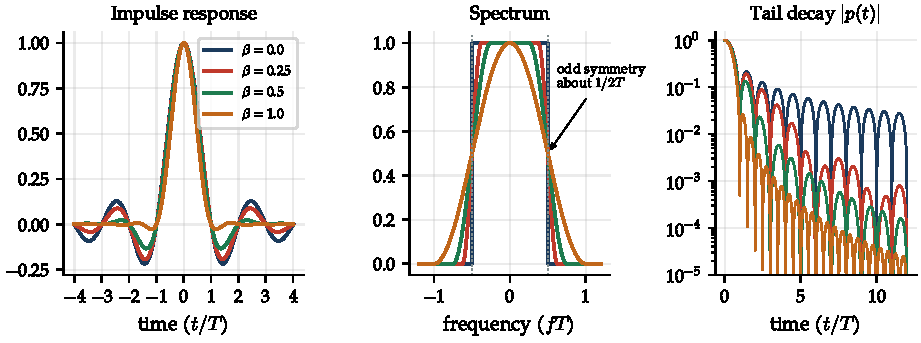
\includegraphics[width=\linewidth]{figs/ch08_raised_cosine}
\end{minipage}\hfill
\begin{minipage}[c]{0.57\linewidth}\centering
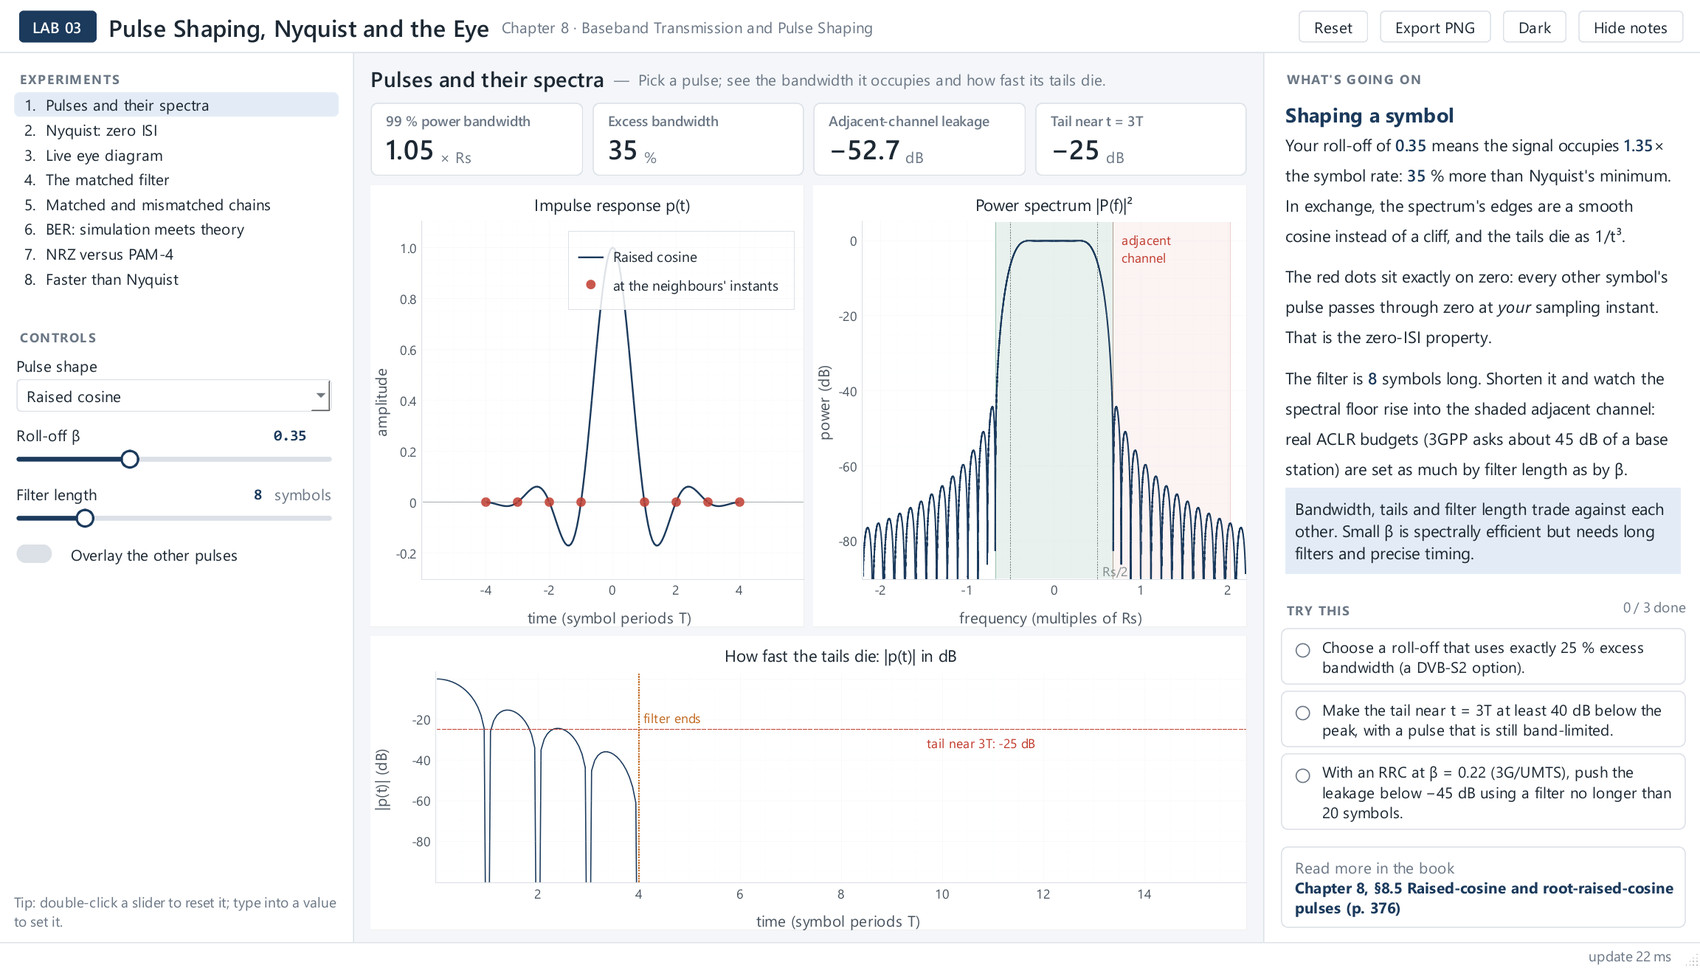
\includegraphics[width=\linewidth]{figs/appB_lab03_pulses}
\end{minipage}
\caption{Same code, two outputs. Left: the raised-cosine figure of Chapter~\ref{ch:baseband}, a
vector PDF drawn by \texttt{ch08\_figs.py}. Right: Lab~3's first experiment, drawn live by the Lab
Studio. Both call \texttt{commlib.filters}, so the curves and the numbers agree by construction.}
\label{fig:appB_twooutputs}
\end{figure}

\begin{inpractice}[The lab author's checklist]
\texttt{LAB\_STYLE\_GUIDE.md} gives the full rules; the essentials are these. Put reusable signal
processing in \texttt{commlib} (a new module if needed) with a test, never in the lab or in
\texttt{studio}. Give each experiment one clear ``aha'', 2--4 readouts with units, and 2--4
challenges that are false at the defaults and require a trade-off; calibrate them with a short
sweep. Keep \texttt{update} under about 50\,ms (budget 20\,000--50\,000 samples) and move anything
slower into \texttt{background}. Fix axis ranges so plots do not jump while a slider moves. Use the
book palette (\texttt{NAVY}, \texttt{RED}, \texttt{GREEN}, \texttt{ORANGE}, \texttt{PURPLE},
\texttt{GRAY}), which maps automatically to the dark theme. Then run
\texttt{python labs/labNN\_name.py -{}-selftest}, look at every screenshot, and add the lab to
\texttt{studio/catalog.py} so the gallery shows it.
\end{inpractice}

%======================================================================
\section{Reproducing the book's figures}
\label{sec:appB:figs}
%======================================================================

\begin{figure}[htbp]\centering
\begin{tikzpicture}[font=\sffamily\footnotesize,
  b/.style={draw=navy,fill=navy!6,thick,rounded corners=2pt,minimum height=1.0cm,minimum width=2.9cm,align=center,inner sep=3pt},
  e/.style={-{Stealth[length=2.3mm]},thick,navy!70},
  l/.style={font=\sffamily\scriptsize,text=black!65,align=center}]
\node[b,fill=accent!10,draw=accent,minimum width=2.2cm] (cl) at (0,0) {\texttt{commlib}};
\node[b] (fs) at (3.9,0.85) {\texttt{chNN\_figs.py}\\{\scriptsize + \texttt{figstyle.py}}};
\node[b] (lab) at (3.9,-0.85) {\texttt{labNN\_*.py}\\{\scriptsize\texttt{-{}-shot file.png}}};
\node[b] (pdf) at (8.3,0.85) {\texttt{figs/chNN\_*.pdf}\\{\scriptsize vector figures}};
\node[b] (png) at (8.3,-0.85) {\texttt{figs/appB\_*}\\{\scriptsize screenshots}};
\node[b] (bk) at (12.6,0) {\texttt{build\_chapter.sh}\\{\scriptsize $\to$ the PDF}};
\draw[e] (fs.west) -- (cl); \draw[e] (lab.west) -- (cl);
\draw[e] (fs) -- node[l,above]{\texttt{save()}} (pdf);
\draw[e] (lab) -- node[l,below]{Qt grab} (png);
\draw[e] (pdf.east) -- (bk); \draw[e] (png.east) -- (bk);
\end{tikzpicture}
\caption{Where the pictures in this book come from. Data figures are drawn by one script per
chapter and screenshots by the labs themselves; both call \texttt{commlib}, and LaTeX includes the
results.}
\label{fig:appB_pipeline}
\end{figure}

\begin{sloppypar}
Every data figure in this book is a vector PDF generated by a Python script, one per chapter, in
\texttt{book/figscripts/}. For example, \texttt{ch08\_figs.py} writes the files
\texttt{book/figs/ch08\_*.pdf}, and \texttt{appA\_figs.py} writes the figures of Appendix~\ref{appA}. Each script begins with
\texttt{from figstyle import *}, which sets the book's fonts and colours, defines the standard figure
widths \texttt{W1} and \texttt{W2} (inches), puts \texttt{commlib} on the path and provides
\texttt{save(fig, name)} (Figure~\ref{fig:appB_pipeline}). Each figure is one function named after the figure, so a figure's file name
tells you where its code is. Figure~\ref{fig:appA_qfunc}, for instance, is the file
\texttt{appA\_qfunc.pdf}, written by the function \texttt{qfunc\_bounds} in \texttt{appA\_figs.py};
the raised-cosine figure of Chapter~\ref{ch:baseband} (left in Figure~\ref{fig:appB_twooutputs}) is
\texttt{ch08\_raised\_cosine.pdf}, written by the function \texttt{raised\_cosine} in
\texttt{ch08\_figs.py}.
\end{sloppypar}

\begin{lstlisting}[language=bash]
cd book/figscripts
python ch08_figs.py          # regenerate all Chapter 8 figures
cd ..
./build.sh figs              # every chNN_figs.py, then the whole book
bash build_chapter.sh ch08   # one chapter in an isolated temporary build
\end{lstlisting}
To change a figure, edit its function, rerun the script and rebuild. Because the scripts call the
same \texttt{commlib} functions as the labs, a figure is also a worked example of the library: copy
the function into a script of your own, replace \texttt{save} with \texttt{plt.show()}, and you
have an interactive Matplotlib version; or turn it into a lab experiment as in
Section~\ref{sec:appB:ownlab}. A few expensive Monte Carlo figures cache their results in
\texttt{figscripts/cache/}; delete the cache file to force a fresh run. The fonts are TeX Gyre
Pagella when it can be found (from TeX Live or MiKTeX) and otherwise fall back to Palatino or DejaVu
Serif, which changes the look slightly but not the content.

\begin{sloppypar}
The screenshots in this appendix were made by the labs themselves, with the same
\texttt{-{}-shot} option you can use: \texttt{python labs/lab03\_pulse\_shaping.py -{}-exp 3
-{}-shot eye.png} opens the experiment, waits for it to draw and saves the window
(with \texttt{QT\_QPA\_PLATFORM=offscreen} it runs without a screen; the images printed here were
grabbed at 1.6 times the normal pixel density for sharpness). The gallery accepts
\texttt{python labs/launcher.py -{}-smoke gallery.png}.
\end{sloppypar}

\mdcpairany{appB_grc}{GNU Radio Companion with a QPSK receiver of the same shape as
\texttt{gr02}: band-edge FLL, polyphase clock synchroniser and Costas loop, with QT GUI sinks
watching the constellation and spectrum between blocks.}{appB_qtgui}{GNU Radio's QT GUI sinks:
time-domain I and Q, a constellation and power spectra of the signals labelled TX (blue) and RX
(red) at two points of a PSK flowgraph, updating live while it runs.}

%======================================================================
\section{GNU Radio and the USRP B200}
\label{sec:appB:gnuradio}
%======================================================================

\subsection{The radio}

The Ettus Research USRP B200 is a single-board, USB-powered software-defined radio built around the
Analog Devices AD9364 RF transceiver (Chapter~\ref{ch:sdr}). It has one transmit and one receive
chain, tunes continuously from 70\,MHz to 6\,GHz and streams up to 56\,MHz of instantaneous
bandwidth over USB~3.0 (Ettus data sheet). Its two SMA ports are labelled \texttt{TX/RX} (transmit, or
receive when not transmitting) and \texttt{RX2} (receive only). The transmit gain control spans
0--89.75\,dB and the receive gain 0--76\,dB. Two figures from the data sheet matter for safety: the
transmit power is specified as more than +10\,dBm (it varies with frequency), and the maximum safe
receive input is $-15$\,dBm. A direct cable from \texttt{TX/RX} to \texttt{RX2} could therefore put
25\,dB or more power into the receiver than it is rated for.

\subsection{Installing GNU Radio}

The scripts in \texttt{gnuradio/} target GNU Radio~3.10 with UHD~4 and were developed with
GNU Radio~3.10.9 on Ubuntu~24.04.

\begin{description}[leftmargin=1.2em,itemsep=3pt,font=\normalfont\bfseries]
\item[radioconda (recommended, all platforms).] radioconda is a conda distribution that bundles GNU
Radio, UHD and other SDR drivers with a matching Python and NumPy. Download the installer for your
platform from its GitHub releases page,
\url{https://github.com/ryanvolz/radioconda}. Install it, open the radioconda prompt and add the lab packages with conda so that NumPy stays consistent:
\begin{lstlisting}[language=bash]
mamba install scipy matplotlib pyside6 pyqtgraph
# fetch the FPGA/firmware images UHD loads into the B200
uhd_images_downloader
# should list the B200 (serial number, type=b200)
uhd_find_devices
# full report; loads the FPGA image the first time
uhd_usrp_probe
\end{lstlisting}
On Windows the B200 also needs a USB driver, and on Linux a udev rule so that ordinary users may open
it; the radioconda and UHD installation guides give the exact steps for each.
\item[Ubuntu and Debian packages.] Install with
\begin{lstlisting}[language=bash]
sudo apt install gnuradio uhd-host
sudo uhd_images_downloader
\end{lstlisting} These packages are built against the distribution's NumPy.
If a newer NumPy has been installed with \texttt{pip} into the same Python, GNU Radio will fail to
import (Section~\ref{sec:appB:trouble}); keep the labs in their own virtual environment.
\item[Windows Subsystem for Linux.] Possible with USB pass-through, but radioconda on native Windows
is simpler for hardware work.
\end{description}

The flowgraphs are plain Python, the same code GNU Radio Companion generates, so they run with
\texttt{python gr02\_psk\_link.py} from the \texttt{gnuradio/} folder. They import \texttt{commlib} from
the parent folder (\texttt{gr05} uses its Viterbi decoder), so keep the repository intact.
GNU Radio Companion, the graphical editor of Figure~\ref{fig:appB_grc}, is the best way to
\emph{see} such a chain; its \emph{QT GUI} sinks (Figure~\ref{fig:appB_qtgui}) are the same kind of
live constellation and spectrum displays the flowgraphs open.

\begin{table}[htbp]\centering\small
\caption{Options shared by all flowgraphs (\texttt{grcommon.base\_parser}).}\label{tab:appB:gropts}
\begin{tabularx}{\linewidth}{@{}>{\ttfamily}l>{\raggedright\arraybackslash}X@{}}
\toprule
\normalfont Option & Meaning\\
\midrule
-{}-args & UHD device arguments (default \texttt{type=b200})\\
-{}-freq & RF centre frequency in Hz (default 915\,MHz)\\
-{}-rate & sample rate in samples per second (per-script default)\\
-{}-tx-gain, -{}-rx-gain & B200 gains in dB (0--89.75 and 0--76); start low\\
-{}-sim & use the software channel instead of the radio\\
-{}-snr & simulation only: SNR per sample in dB (default 20)\\
-{}-cfo & carrier offset in Hz; on hardware it is applied as an RX local-oscillator offset\\
-{}-ppm & simulation only: sample-clock offset in parts per million\\
-{}-multipath & simulation only: add the three-tap channel\\
-{}-nogui & no Qt windows; print statistics to the console\\
-{}-duration & stop after this many seconds (0 runs until Ctrl-C)\\
\bottomrule
\end{tabularx}
\end{table}

\subsection{Common options and simulation mode}

All five scripts share the command-line options in Table~\ref{tab:appB:gropts}, defined in
\texttt{grcommon.py}. The most important is \texttt{-{}-sim}: it replaces the B200 by GNU Radio's
\texttt{channel\_model} block preceded by a throttle, adding white noise at the requested SNR per
sample, a carrier offset (\texttt{-{}-cfo}), a sample-clock offset (\texttt{-{}-ppm}) and, with
\texttt{-{}-multipath}, the three-path channel $[1,\,0,\,0.35+0.25j,\,0,\,-0.15]$ (taps at 0, 2 and 4
samples). Every experiment should be run in simulation first: if it does not work there, it will not
work over the air. With \texttt{-{}-nogui} the scripts print statistics to the console instead of
opening Qt windows, and \texttt{-{}-duration} stops them after a fixed time, which makes them usable in
scripts and on headless machines.

\subsection{The five flowgraphs}

\begin{figure}[htbp]\centering
\begin{tikzpicture}[font=\sffamily\scriptsize,
  b/.style={draw=navy,fill=navy!6,thick,rounded corners=2pt,minimum height=0.9cm,minimum width=1.45cm,align=center,inner sep=2pt},
  e/.style={-{Stealth[length=2mm]},thick,navy!70},
  l/.style={font=\sffamily\scriptsize,text=black!65,align=center}]
\node[b,fill=accent!10,draw=accent] (src) at (0,0) {B200\\or \texttt{-{}-sim}};
\node[b] (agc) at (1.85,0) {AGC};
\node[b] (fll) at (3.7,0) {band-edge\\FLL};
\node[b] (pfb) at (5.55,0) {PFB clock\\sync (32 RRC)};
\node[b] (cma) at (7.4,0) {CMA\\equaliser};
\node[b] (cos) at (9.25,0) {Costas\\loop};
\node[b] (dec) at (11.1,0) {slicer +\\diff.\ decode};
\node[b,fill=practc!8,draw=practc] (ber) at (12.95,0) {BER\\counter};
\foreach \a/\b in {src/agc,agc/fll,fll/pfb,pfb/cma,cma/cos,cos/dec,dec/ber} \draw[e] (\a) -- (\b);
\node[l] at (3.7,-0.85) {coarse\\frequency};
\node[l] at (5.55,-0.85) {symbol\\timing};
\node[l] at (7.4,-0.85) {multipath,\\15 taps};
\node[l] at (9.25,-0.85) {fine\\phase};
\node[l] at (11.1,-0.85) {removes the\\$90^\circ$ ambiguity};
\node[l] at (12.95,-0.85) {aligns to the\\known pattern};
\end{tikzpicture}
\caption{The receiver chain of \texttt{gr02\_psk\_link.py}, the textbook synchronisation sequence of
Chapter~\ref{ch:sync} in eight blocks. The GUI shows the constellation after each stage, so you can
see what every block contributes.}
\label{fig:appB_gr02}
\end{figure}

\paragraph{\texttt{gr01\_spectrum\_iq\_capture.py}: spectrum, waterfall and IQ recording
(Chapters~\ref{ch:signals} and~\ref{ch:sdr}).} A receive-only script: it never transmits. It shows a
4096-point spectrum and a waterfall with sliders for centre frequency (70\,MHz to 6\,GHz) and receive
gain, and with \texttt{-{}-nogui} prints the mean power in dBFS once a second. With \texttt{-{}-out
file.cfile} it records complex-float samples (with \texttt{-{}-duration}, a fixed number of them) and
writes a SigMF \texttt{.sigmf-meta} sidecar describing the rate and frequency; load the recording with
\texttt{commlib.read\_cfile} as in Lab~1. \texttt{-{}-no-dc-corr} turns off UHD's automatic DC-offset
correction so that you can see the zero-IF receiver's DC spur (Chapter~\ref{ch:sdr}). In simulation it
synthesises two tones 20\,dB apart, an IQ-imbalance image 30\,dB below the stronger tone, an optional
DC term and noise, the impairments Lab~1 teaches you to recognise.
\begin{lstlisting}[language=bash]
# FM broadcast band
python gr01_spectrum_iq_capture.py --freq 100e6 --rate 2e6
python gr01_spectrum_iq_capture.py --freq 915e6 --duration 5 \
       --out ../data/capture.cfile
python gr01_spectrum_iq_capture.py --sim --nogui --duration 3 --out sim.cfile
\end{lstlisting}

\mdcpairany{appB_lab01_waterfall}{Rehearse before you record: Lab~1's \emph{live waterfall} of a
crowded band (an FM station, CW beacons, TDMA bursts, a frequency hopper and a chirp radar) is what
gr01 shows you on real air; change the FFT size and window and see what you can resolve.}{appB_lab04_costas}{Lab~4's
\emph{Costas loop locks on}: the same loop that ends gr02's receiver chain, pulling a spinning QPSK
ring into four clusters. Try the loop bandwidths here before you try them on the B200.}

\paragraph{\texttt{gr02\_psk\_link.py}: a complete QPSK link (Chapters~\ref{ch:modulation},
\ref{ch:sync} and~\ref{ch:equalization}).} The transmitter sends a repeating block of 1024
pseudo-random bytes as differentially encoded QPSK with root-raised-cosine shaping ($\beta=0.35$,
four samples per symbol by default). The receiver (Figure~\ref{fig:appB_gr02}) is a textbook chain: AGC; a band-edge FLL for
coarse frequency correction; a polyphase-filterbank clock synchroniser (32 RRC matched filters) for
timing; a 15-tap fractionally spaced CMA equaliser; a Costas loop for fine phase; a slicer;
differential decoding, which removes the Costas loop's $90^\circ$ ambiguity; and a BER counter that
aligns itself to the known pattern by circular correlation. The GUI overlays the constellation after
each stage so you can see what every block contributes, shows the spectrum before and after the FLL
and the Costas loop's frequency estimate, and has a slider for the Costas loop bandwidth. Options
\texttt{-{}-sps}, \texttt{-{}-amplitude}, \texttt{-{}-fll-bw}, \texttt{-{}-timing-bw}, \texttt{-{}-phase-bw} and
\texttt{-{}-cma-mu} expose every loop. In simulation the link converged to a BER below $10^{-4}$ with a
2\,kHz offset at 18\,dB SNR.
\begin{lstlisting}[language=bash]
python gr02_psk_link.py --sim --cfo 2000 --multipath --ppm 50 --snr 15
# headless BER measurement
python gr02_psk_link.py --sim --nogui --duration 10
# hardware, cabled loopback
python gr02_psk_link.py --cfo 2000
\end{lstlisting}

\begin{figure}[htbp]\centering
\begin{tikzpicture}[font=\sffamily\small,
  att/.style={draw=accent,fill=accent!8,thick,minimum height=1.0cm,minimum width=2.0cm,align=center},
  arr/.style={-{Stealth[length=2.5mm]},thick,navy}]
\node[draw=navy,fill=navy!6,thick,minimum height=3.0cm,minimum width=2.8cm,align=center] (b200) at (0,0)
  {USRP B200\\[3pt]{\footnotesize to host PC}\\{\footnotesize over USB 3.0}};
\coordinate (tx) at (1.4,0.8);
\coordinate (rx) at (1.4,-0.8);
\fill[navy] (tx) circle (2.2pt); \fill[navy] (rx) circle (2.2pt);
\node[anchor=south east,font=\sffamily\footnotesize] at ([xshift=-2pt]tx) {TX/RX};
\node[anchor=north east,font=\sffamily\footnotesize] at ([xshift=-2pt]rx) {RX2};
\node[att] (a1) at (4.0,0.8) {30\,dB\\attenuator};
\node[att] (a2) at (7.0,0.8) {30\,dB\\attenuator};
\draw[arr] (tx) -- (a1);
\draw[arr] (a1) -- (a2);
\draw[arr] (a2.east) -- ++(0.7,0) |- (rx);
\node[align=left,text=accent,font=\sffamily\footnotesize,anchor=north west] at (2.4,-1.05)
  {TX output up to about $+10$\,dBm; RX safe input about $-15$\,dBm\\
   $\Rightarrow$ at least 30\,dB of attenuation, 60\,dB preferred};
\end{tikzpicture}
\caption{Cabled loopback for the B200 experiments. Connect \texttt{TX/RX} to \texttt{RX2} only through
fixed attenuators: at least 30\,dB, and 60\,dB (two 30\,dB pads) for comfort. A single B200 shares one
reference oscillator between transmitter and receiver, so the loopback carrier offset is essentially
zero; use \texttt{-{}-cfo} to inject one.}
\label{fig:appB_loopback}
\end{figure}

\paragraph{\texttt{gr03\_channel\_sounder.py}: a correlation channel sounder
(Chapter~\ref{ch:channels}).} The transmitter repeats a Zadoff--Chu sequence (length 255, root 7 by
default). Because its periodic autocorrelation is a perfect impulse, the receiver's matched filter
output, squared and cut into one vector per period, is the channel's power-delay profile. The script
averages the profiles exponentially, aligns them on the strongest tap, displays the result in dB and
every two thousand periods prints the taps within 20\,dB of the peak and the RMS delay spread; with
\texttt{-{}-out} it saves the averaged profile as a NumPy file. The delay resolution is one sample
($1/\text{rate}$: 100\,ns at the default 10\,MS/s) and the longest unambiguous excess delay is 255
samples. In simulation with \texttt{-{}-multipath} it recovers the three-tap profile and reports an RMS
delay spread of 88\,ns, the value you can compute by hand from the taps. In cabled loopback it shows a
single tap: your system's own impulse response, which you should remember to subtract when you
later use antennas.

\paragraph{\texttt{gr04\_ofdm\_link.py}: packet OFDM (Chapter~\ref{ch:ofdm}).} This script wraps GNU
Radio's reference OFDM transceiver (\texttt{ofdm\_tx}/\texttt{ofdm\_rx}): a 64-point FFT with a 16-sample
cyclic prefix, 48 data and 4 pilot subcarriers, Schmidl--Cox synchronisation, a BPSK header and a
payload of BPSK, QPSK or 8-PSK (\texttt{-{}-bps 1}, \texttt{2} or \texttt{3}), each packet protected by a
CRC-32. The transmitter cycles through 64 numbered 96-byte packets, separated by 160 zero samples so
that the detector resets between bursts. The receiver checks the CRC, the content and the sequence
numbers and reports packet error rate and goodput every second. In simulation it delivered every
packet at 20\,dB SNR and about 99\% with multipath and a 5\,kHz offset. Things to try: raise
\texttt{-{}-bps} to 3 and find the SNR at which the packet error rate collapses; add multipath and note
that no equaliser beyond the one-tap-per-subcarrier correction is needed because the cyclic prefix
is longer than the channel; push \texttt{-{}-cfo} beyond half a subcarrier spacing ($\text{rate}/128$)
and watch synchronisation fail.

\paragraph{\texttt{gr05\_coded\_link.py}: measured coding gain (Chapters~\ref{ch:classiccodes}
and~\ref{ch:sync}).} Each frame carries 500 information bits encoded by the industry-standard $K=7$,
rate-$\tfrac12$ (133,\,171) convolutional code from \texttt{commlib}, sent as 1012 BPSK symbols in 22
blocks, each preceded by 16 pilot symbols, after a 63-symbol m-sequence preamble. The receiver runs
an AGC, a narrow FLL and the polyphase clock synchroniser, then a Python block that finds the
preamble by correlation, estimates the carrier phase from each pilot group and interpolates it across
the data, estimates $E_s/N_0$, counts raw channel errors and decodes with soft-decision Viterbi. It
prints $E_s/N_0$, raw BER, decoded BER and frame error rate, so you can place your operating point on
the curves of Lab~8. Pilots replace a Costas loop because the code works near $E_s/N_0=0$\,dB, where
a decision-directed loop slips cycles constantly: the same reason DVB-S2 and 5G NR use pilots
(Chapter~\ref{ch:sync}). In simulation, \texttt{-{}-snr} is per sample; with four samples per symbol
$E_s/N_0$ is 6\,dB higher and $E_b/N_0$ another 3\,dB higher. At $E_s/N_0=2.9$\,dB the simulated link
measured a raw BER of $2.4\times10^{-2}$ (theory $2.3\times10^{-2}$) and no decoded errors.

\subsection{Safety and the law}

\mdcpairany{appB_lab15_tune}{Lab~15, \emph{Tune the superhet}: the simulated medium-wave band, the
preselector and the 455\,kHz IF of a classic receiver. Recording a real broadcast band with gr01 and
finding the same structure in it is the hardware companion.}{appB_lab05_sounder}{Lab~5,
\emph{Sounding a channel}: a Zadoff--Chu sequence correlated against six echoes, the simulated twin
of \texttt{gr03\_channel\_sounder.py}; compare its power-delay profile with what your own cable
channel measures.}

\begin{table}[htbp]\centering\footnotesize
\caption{Suggested B200 experiments. ``Loopback'' means the attenuated cable of Figure~\ref{fig:appB_loopback}.}\label{tab:appB:hwexp}
\renewcommand{\arraystretch}{1.15}
\begin{tabularx}{\linewidth}{@{}l>{\raggedright\arraybackslash}X>{\raggedright\arraybackslash}p{0.2\linewidth}@{}}
\toprule
Ch. & Experiment & Tools\\
\midrule
2, 7 & Record a few seconds of the FM band and of a quiet band; find the DC spur (\texttt{-{}-no-dc-corr}) and the IQ image of a strong station; estimate and correct the imbalance offline & gr01, Lab 1\\
3 & Terminate \texttt{RX2} in 50\,$\Omega$ and measure the noise level in dBFS versus receive gain; relate it to $-174$\,dBm/Hz, the bandwidth and the receiver's noise figure; check that the samples are Gaussian & gr01, Labs 1, 33\\
4 & Record an FM broadcast station at 1--2\,MS/s; demodulate it offline with the discriminator of Lab 14 and find the 19\,kHz pilot, the 38\,kHz stereo subcarrier and the 57\,kHz RDS signal & gr01, Lab 14\\
5, 6 & Decimate a wideband recording to one channel with a multistage DDC; compare CIC-plus-compensator and single-stage FIR designs on real data & gr01, Lab 17\\
8, 9 & Edit the transmit roll-off in gr02 so that TX and RX filters mismatch and watch the constellation spread; measure the transmitted spectrum and its shoulders & gr02, gr01, Lab 3\\
10 & Sweep \texttt{-{}-cfo} until the FLL loses lock; vary the Costas bandwidth while watching phase jitter and cycle slips & gr02, Lab 4\\
11 & Build a known two-path channel from a power splitter and two cables of different lengths (about 5\,ns of delay per metre of typical coax) and measure it with the sounder; with a licence, measure indoor profiles & gr03, Lab 5\\
12 & Run gr02 through the two-path cable channel and watch the CMA equaliser open the eye & gr02, Lab 6\\
14, 15 & Lower \texttt{-{}-tx-gain} in gr05 until raw errors appear; compare raw and decoded BER with Lab 8's curves & gr05, Lab 8\\
17 & Measure packet error rate versus modulation, gain and injected offset; compare with Lab 7 & gr04, Lab 7\\
18 & With an active GPS antenna and an external bias tee, record L1 (1575.42\,MHz) at 4\,MS/s and acquire satellites with \texttt{spread.acquire}; widen the Doppler search to cover the B200 oscillator's error & gr01, Lab 25\\
21 & Record a cellular downlink carrier (receive only) and find PSS/SSS to recover the physical cell identity & gr01, Lab 27\\
22 & Record the BLE advertising channels or Wi-Fi beacons at 2.4\,GHz and detect preambles; dechirp a LoRa transmission from your own device & gr01, Lab 31\\
23 & Record a low-Earth-orbit amateur or weather satellite pass at VHF/UHF and compare the measured Doppler curve with \texttt{satellite.leo\_pass} & gr01, Lab 18\\
\bottomrule
\end{tabularx}
\end{table}

\begin{pitfall}[Never connect TX directly to RX]
The B200's transmitter can deliver more power than its receiver can survive. Always use the cabled
loopback of Figure~\ref{fig:appB_loopback} with at least 30\,dB of attenuation (60\,dB is safer, and
the receive gain has range to spare), start with a low \texttt{-{}-tx-gain} and raise it slowly while
watching the received level, and keep a 50\,$\Omega$ load or attenuator on any transmit port that is
active. Discharge static before handling the SMA connectors.
\end{pitfall}

Cabled experiments radiate essentially nothing and need no licence. \emph{Radiating} is different:
every transmission is regulated by the national administration under the ITU Radio Regulations, and
an SDR has not been certified as a transmitter for any particular service. In practice:
\begin{itemize}[leftmargin=1.5em,itemsep=2pt]
\item Transmit over the air only where you are clearly entitled to: under an amateur radio licence,
on amateur frequencies and within its rules (station identification, power limits, no obscured
content), under an experimental licence, or, where national rules allow it, at the very low powers
permitted in licence-exempt bands. Typical examples are 902--928\,MHz and 2400--2483.5\,MHz in ITU
Region~2 (in the USA, FCC Part~15) and the short-range-device bands 433.05--434.79\,MHz and
863--870\,MHz in Europe (ERC Recommendation 70-03), which come with power and duty-cycle limits. The
scripts default to 915\,MHz; in Region~1 use \texttt{-{}-freq 433.92e6} or \texttt{868e6}. Check your own
country's rules before radiating anything.
\item Never transmit in bands used for navigation, aviation, emergency services or cellular
networks. A few milliwatts at 1575\,MHz can jam GPS receivers nearby.
\item Receiving is permitted almost everywhere, but many jurisdictions restrict intercepting, recording
or disclosing the content of other people's communications. The receive experiments below use public
broadcasts, beacons and synchronisation signals; keep it that way.
\end{itemize}

\subsection{Hardware experiments by chapter}

Table~\ref{tab:appB:hwexp} suggests an experiment for most chapters. Receive-only experiments need an
antenna suited to the band; transmit experiments use the cabled loopback unless you hold the right
licence. The lab named in the last column is the place to rehearse each experiment in simulation
first, and to analyse your recordings afterwards.

%======================================================================
\section{Troubleshooting}
\label{sec:appB:trouble}
%======================================================================

Most problems fall into four families: Qt cannot open a window, the window is the wrong size, the
code runs slowly, or GNU Radio and the labs disagree about NumPy. Table~\ref{tab:appB:trouble}
and its two continuations list the symptoms people actually meet and their fixes. When in doubt, run the self-test of one
lab (\texttt{python tests/selftest\_labs.py lab03}): it uses no screen, so if it passes the
library and the labs are fine and the problem is in the display setup.

\begin{table}[htbp]\centering\footnotesize
\caption{Common problems and their fixes.}\label{tab:appB:trouble}
\renewcommand{\arraystretch}{1.2}
\begin{tabularx}{\linewidth}{@{}>{\raggedright\arraybackslash}p{0.28\linewidth}>{\raggedright\arraybackslash}X@{}}
\toprule
Symptom & Cause and fix\\
\midrule
\multicolumn{2}{@{}l}{\textit{Installing and starting}}\\
\texttt{ModuleNotFoundError: PySide6} or \texttt{pyqtgraph} & The requirements were installed into a different Python. Activate the virtual environment first, or run \texttt{python -m pip install -r moderncomms-labs/requirements.txt} with the same \texttt{python} you use to start the labs.\\
\texttt{ModuleNotFoundError: commlib} or \texttt{studio} & A copied lab file has lost its neighbour \texttt{labs/\_path.py}. Run labs from their own folder (or the repository root) and keep \texttt{moderncomms-labs/} intact.\\
Linux: \texttt{qt.qpa.plugin: Could not load the Qt platform plugin "xcb"} & Qt~6 needs \texttt{libxcb-cursor0} (\texttt{sudo apt install libxcb-cursor0}); on a server without a display use the self-test or \texttt{QT\_QPA\_PLATFORM=offscreen}.\\
\bottomrule
\end{tabularx}
\end{table}

\begin{table}[htbp]\centering\footnotesize
\caption{Common problems and their fixes: the display.}\label{tab:appB:trouble3}
\renewcommand{\arraystretch}{1.2}
\begin{tabularx}{\linewidth}{@{}>{\raggedright\arraybackslash}p{0.28\linewidth}>{\raggedright\arraybackslash}X@{}}
\toprule
Symptom & Cause and fix\\
\midrule
\multicolumn{2}{@{}l}{\textit{Display}}\\
No window over SSH or in a container & There is no display. The self-test, \texttt{-{}-shot} and \texttt{-{}-smoke} work with \texttt{QT\_QPA\_PLATFORM=offscreen} (the self-test sets it itself), and Windows~11's WSLg provides a display for WSL.\\
Window too large or too small on a high-resolution screen & The labs follow the operating system's scaling. To override it, set \texttt{QT\_SCALE\_FACTOR} (for example \texttt{1.25} or \texttt{0.9}) before starting a lab. On Windows check \emph{Display\,$\to$\,Scale}; on Linux/X11 also \texttt{QT\_SCREEN\_SCALE\_FACTORS}.\\
Text missing or boxes instead of letters in offscreen screenshots & Offscreen Qt has no fonts of its own; the Lab Studio points it at the system font folder automatically on Windows and macOS. On Linux install a font package (e.g.\ \texttt{fonts-dejavu}) or set \texttt{QT\_QPA\_FONTDIR}.\\
Plots look wrong after a theme change, or the window opens on an odd experiment & Settings (theme, last experiment, completed challenges) are stored with QSettings under \emph{ModernComms/LabStudio}. \textsf{Reset} restores an experiment; \texttt{-{}-exp N} chooses the page.\\
No sound from \textsf{Listen} & Install \texttt{sounddevice} (\texttt{pip install sounddevice}), or on Linux make sure \texttt{paplay} or \texttt{aplay} exists. The rest of the lab works without sound.\\
\textsf{Read more in the book} opens the PDF at page 1 & Your PDF viewer cannot be told a page portably; the status bar names the page. Install \texttt{pypdf} for exact pages in browsers, SumatraPDF or Adobe Reader, and make sure \texttt{book/main.pdf} exists.\\
\bottomrule
\end{tabularx}
\end{table}

\begin{table}[htbp]\centering\footnotesize
\caption{Common problems and their fixes (continued).}\label{tab:appB:trouble2}
\renewcommand{\arraystretch}{1.2}
\begin{tabularx}{\linewidth}{@{}>{\raggedright\arraybackslash}p{0.28\linewidth}>{\raggedright\arraybackslash}X@{}}
\toprule
Symptom & Cause and fix\\
\midrule
\multicolumn{2}{@{}l}{\textit{Speed}}\\
A lab with small matrix solves (equalisers, MIMO) runs 10--100 times slower than expected on a many-core machine & OpenBLAS thread start-up and contention. \texttt{labs/\_path.py} sets \texttt{OPENBLAS\_NUM\_THREADS}, \texttt{OMP\_NUM\_THREADS} and \texttt{MKL\_NUM\_THREADS} to 2 before NumPy is imported; if you import NumPy yourself first (in your own scripts), set them in the shell instead.\\
Sliders feel sluggish & Close other labs that are playing animations, pause Play, or choose a quicker setting where the lab offers one (``Quick'' Monte Carlo effort). The status bar shows the update time; above a few hundred milliseconds something is wrong.\\
Monte Carlo curves stop at $10^{-3}$ or $10^{-4}$ & The simulation ran out of trials before seeing errors. Choose the thorough effort or wait longer; the floor is the simulation's resolution, not the code's.\\
\midrule
\multicolumn{2}{@{}l}{\textit{Text and figures}}\\
Garbled characters or \texttt{UnicodeEncodeError} on Windows & The console is using a legacy code page. The labs reconfigure their output to UTF-8; for your own scripts set \texttt{PYTHONIOENCODING=utf-8}.\\
Figures use a different font from the book & \texttt{figstyle.py} looks for TeX Gyre Pagella in the TeX Live and MiKTeX font folders and falls back to Palatino or DejaVu Serif. Install the \texttt{tex-gyre} fonts (or edit the glob in \texttt{figstyle.py}) and delete Matplotlib's font cache.\\
\midrule
\multicolumn{2}{@{}l}{\textit{GNU Radio and the B200}}\\
\texttt{from gnuradio import gr} fails with an ``initialization failed'' or NumPy ABI error & Distribution GNU Radio packages are compiled against NumPy~1.x; a \texttt{pip}-installed NumPy~2.x in the same Python breaks them. Use radioconda, run the flowgraphs with the system packages first on the path (e.g.\ \texttt{PYTHONPATH=/usr/lib/python3/dist-packages python3 gr02\_psk\_link.py}), or keep the labs in a separate virtual environment. The labs themselves work with NumPy 1.24+ and 2.x.\\
\texttt{uhd\_find\_devices} finds nothing & Check the USB~3.0 cable and port, the Windows USB driver or Linux udev rule, and that \texttt{uhd\_images\_downloader} has been run.\\
The console fills with \texttt{O} (or \texttt{U}) characters & UHD reports receive overflows (or transmit underflows): the host cannot keep up. Lower \texttt{-{}-rate}, close the GUI (\texttt{-{}-nogui}), use a USB~3.0 port and avoid virtual machines.\\
Flowgraph Qt windows fail to open & GNU Radio's GUI uses PyQt5 (not the labs' PySide6): it is missing, or there is no display. Use \texttt{-{}-nogui}.\\
The hardware link never locks but \texttt{-{}-sim} works & Check the loopback wiring and attenuation, raise \texttt{-{}-tx-gain} in small steps, and look at the raw spectrum with gr01 at the same frequency to confirm the signal is there and not clipped.\\
\bottomrule
\end{tabularx}
\end{table}

\FloatBarrier
\furtherreading
\begin{itemize}
\item The GNU Radio project, \emph{GNU Radio Wiki and Tutorials}, \url{https://wiki.gnuradio.org}. Start
with the beginner tutorials and the pages on the \texttt{digital} module's synchronisation blocks
used in gr02 and gr05.
\item Ettus Research, \emph{USRP Hardware Driver and USRP Manual}, \url{https://files.ettus.com/manual/},
and the B200/B210 product data sheet: installation, device arguments, gain ranges and RF limits.
\item R.~Volz, \emph{radioconda}, \url{https://github.com/ryanvolz/radioconda}. Installers and
platform notes, including USB drivers and permissions.
\item M.~Lichtman, \emph{PySDR: A Guide to SDR and DSP using Python}, \url{https://pysdr.org}. A free
online companion that covers much of the same ground in a hands-on style, including the USRP.
\item T.~F.~Collins, R.~Getz, D.~Pu and A.~M.~Wyglinski, \emph{Software-Defined Radio for Engineers},
Artech House, 2018. SDR hardware and receiver algorithms built around the AD936x family used in the
B200.
\item \emph{SigMF: the Signal Metadata Format}, \url{https://github.com/sigmf/SigMF}. The specification
behind the \texttt{.sigmf-meta} files written by gr01.
\item The Qt for Python (PySide6) documentation, \url{https://doc.qt.io/qtforpython-6/}, and the
pyqtgraph documentation, \url{https://pyqtgraph.readthedocs.io}: the two libraries under the Lab
Studio, for readers who want to extend it.
\item ITU, \emph{Radio Regulations} (current edition); for the USA, 47 CFR Part~15 (licence-exempt
devices) and Part~97 (amateur service); for Europe, ERC Recommendation 70-03 on short-range devices.
The rules you must know before radiating anything.
\end{itemize}
